\documentclass[12pt]{article}
\usepackage{amsmath}
\usepackage{amsfonts}
\usepackage{float}
\usepackage{fancyhdr}
\usepackage{graphicx}
\usepackage{setspace}
\usepackage[colorlinks=true,linkcolor=blue, citecolor=red]{hyperref}
\usepackage{url}
\usepackage[top=.75in, left=.75in, right=.75in, bottom=1in]{geometry}

% For algorithm
\usepackage{algorithm}
\usepackage{algpseudocode}

% ============ CODE ============
\usepackage{listings}
\usepackage{xcolor}
\definecolor{codegreen}{rgb}{0,0.6,0}
\definecolor{codegray}{rgb}{0.5,0.5,0.5}
\definecolor{codepurple}{rgb}{0.58,0,0.82}
\definecolor{backcolour}{rgb}{0.95,0.95,0.92}

% Styling for the code.
\lstdefinestyle{mystyle}{
    backgroundcolor=\color{backcolour},   
    commentstyle=\color{codegreen},
    keywordstyle=\color{magenta},
    numberstyle=\tiny\color{codegray},
    stringstyle=\color{codepurple},
    basicstyle=\ttfamily\footnotesize,
    breakatwhitespace=false,         
    breaklines=true,                 
    captionpos=b,                    
    keepspaces=true,                 
    numbers=left,                    
    numbersep=5pt,                  
    showspaces=false,                
    showstringspaces=false,
    showtabs=false,                  
    tabsize=2
}
\lstset{style=mystyle}

% Table packages and Unicode / Font support
\usepackage{array}
\usepackage{longtable}
\usepackage{enumitem}
\usepackage{booktabs}
\graphicspath{{../../templates/}{figures/}{./}}
\setlength{\emergencystretch}{3em}
\setlist[enumerate]{label=\arabic*.,leftmargin=*}
\setlist[itemize]{leftmargin=*}

\usepackage{iftex}
\ifPDFTeX
  \usepackage[T1]{fontenc}
  \usepackage[utf8]{inputenc}
  \usepackage{lmodern}
\else
  \usepackage{fontspec}
  \setmainfont{DejaVu Serif}
  \setsansfont{DejaVu Sans}
  \setmonofont{DejaVu Sans Mono}
\fi

% ============ HEADER AND FOOTER ============
% Header length
\setlength{\headheight}{29.43912pt}

% Footer page number would be on the lower-right corner
\pagestyle{fancy}
\fancyfoot{}
\fancyfoot[R]{Page \thepage}

% Disable indentation on new paragraphs
\setlength{\parindent}{0pt}

% Line spacing 1.5
\renewcommand{\baselinestretch}{1.5}

% Define course name, report name and report title.
\newcommand{\coursename}{Introduction of Software Engineering}
\newcommand{\reportname}{Studitopia}
\newcommand{\reporttitle}{\href{https://github.com/RoundFloor/Studitopia.git}{Studitopia}}

\newcommand{\studentname}{%
Nguyen Thanh An (24125024)\\
Nguyen Chi Bao (24125025)\\
Tran Nguyen Khanh Binh (24125026)\\
Tran Canh Anh Tuan (24125048)\\
Nguyen Le Quoc Huy (24125100)
}
\newcommand{\teachername}{Ho Tuan Thanh, Nguyen Ngoc Minh Thu}

% Header
\lhead{\reporttitle}
\rhead{
University of Science - VNUHCM\\
\coursename
}

% Footer
\newcommand{\leftfooter}{}
\lfoot{\leftfooter}

% ============ DOCUMENT ============
\begin{document}

\pagenumbering{roman}
\begin{titlepage}
\begin{spacing}{1.0}
\newcommand{\HRule}{\rule{\linewidth}{0.5mm}}
\centering

\textsc{\LARGE VNU-HCM}\\[0.5cm]
\textsc{\Large University of Science}\\[0.5cm]
\textsc{\large Faculty of Information Technology}\\[0.5cm]
\textsc{Computer Science}\\[0.5cm]

\HRule \\[0.4cm]
{ 
\huge{\bfseries{\reporttitle}}\\[0.5cm]
\large{\bfseries{Project: \reportname}}
}\\[0.4cm]
\HRule \\[0.5cm]

\textbf{\large Subject: \coursename}\\[0.5cm]

\begin{minipage}[t]{0.55\textwidth}
\begin{flushleft} \large
\emph{Students:}\\
\studentname
\end{flushleft}
\end{minipage}
~
\begin{minipage}[t]{0.4\textwidth}
\begin{flushright} \large
\emph{Supervising Teachers:} \\
\teachername
\end{flushright}
\end{minipage}\\[1cm]

{\large \today}\\[1cm]


\includegraphics[scale=.20]{img/hcmus-logo.png}\\[1cm] 

\vfill
\end{spacing}
\end{titlepage}	

\tableofcontents
\pagebreak

\pagenumbering{arabic}
\setcounter{page}{1}

% ============ MARKDOWN CONTENT: PA3/use_case.md ============
\hypertarget{sec:use-case-specification-studitopia-core-use-cases}{}
\section*{Use-Case Specification: Studitopia Core Use Cases}
\par\medskip
\textbf{Company:} \texttt{Studitopia}
\par\medskip
\textbf{Project:} \texttt{Studitopia}
\par\medskip
\textbf{Document:} Use-Case Specification: Core Use Cases UC-01 to UC-07
\par\medskip
\textbf{Version:} \texttt{1.0}
\par\medskip
\hypertarget{sec:document-information}{}
\addcontentsline{toc}{section}{Document Information}
\section*{Document Information}
\par\medskip
\begingroup
\small
\renewcommand{\baselinestretch}{1.0}\selectfont
\renewcommand{\arraystretch}{1.15}
\setlength{\tabcolsep}{6pt}
\begin{longtable}{|>{\raggedright\arraybackslash}p{0.28\textwidth}|>{\raggedright\arraybackslash}p{0.67\textwidth}|}
\hline
\textbf{Field} & \textbf{Value} \\ \hline
\endhead
Project Name & Studitopia \\ \hline
Use-Case Specification & Core Use Cases UC-01 to UC-07 \\ \hline
Version & 1.0 \\ \hline
Date & 14/Nov/2026 \\ \hline
Document Identifier & PA3-G5-UC-SPEC \\ \hline
\end{longtable}
\endgroup
\par\medskip
\hypertarget{sec:revision-history}{}
\addcontentsline{toc}{section}{Revision History}
\section*{Revision History}
\par\medskip
\begingroup
\small
\renewcommand{\baselinestretch}{1.0}\selectfont
\renewcommand{\arraystretch}{1.15}
\setlength{\tabcolsep}{6pt}
\begin{longtable}{|>{\raggedright\arraybackslash}p{0.12\textwidth}|>{\raggedright\arraybackslash}p{0.12\textwidth}|>{\raggedright\arraybackslash}p{0.5\textwidth}|>{\raggedright\arraybackslash}p{0.2\textwidth}|}
\hline
\textbf{Date} & \textbf{Version} & \textbf{Description} & \textbf{Author} \\ \hline
\endhead
10/11 & 1.0 & Filled the RUP use-case template with the seven selected PA3 use cases, including use-case diagrams and specifications & Nguyen Le QUoc Huy \\ \hline
11/11 & 1.0 & Clean all use-case diagram redundance & Nguyen Le Quoc Huy \\ \hline
\end{longtable}
\endgroup
\par\medskip
\hypertarget{sec:document-contribution}{}
\addcontentsline{toc}{section}{Document Contribution}
\section*{Document Contribution}
\par\medskip
\begingroup
\small
\renewcommand{\baselinestretch}{1.0}\selectfont
\renewcommand{\arraystretch}{1.15}
\setlength{\tabcolsep}{6pt}
\begin{longtable}{|>{\raggedright\arraybackslash}p{0.46\textwidth}|>{\raggedright\arraybackslash}p{0.16\textwidth}|>{\raggedright\arraybackslash}p{0.16\textwidth}|>{\raggedright\arraybackslash}p{0.16\textwidth}|}
\hline
\textbf{Use Case} & \textbf{Performed by} & \textbf{Reviewed by} & \textbf{Edited by} \\ \hline
\endhead
UC-01 Register Account and Verify University Email & An & Bảo & An \\ \hline
UC-02 Log In & Huy & Tuấn & Huy \\ \hline
UC-03 Browse and Search the University Forum & Bảo & Huy & Bảo \\ \hline
UC-04 Create Discussion Post & Tuấn & Bình & Tuấn \\ \hline
UC-05 Comment and Answer & Bình & An & Bình \\ \hline
UC-06 Share Learning Resource & Bình & Bảo & Bình \\ \hline
UC-07 Join or Create a Study Room & An & Tuấn & Tuấn \\ \hline
\end{longtable}
\endgroup
\par\medskip
\par\noindent\rule{\linewidth}{0.4pt}\par\medskip
\hypertarget{sec:1-uc-01-register-account-and-verify-university-email}{}
\hypertarget{1-uc-01-register-account-and-verify-university-email}{}
\addcontentsline{toc}{section}{1. UC-01 Register Account and Verify University Email}
\section*{1. UC-01 Register Account and Verify University Email}
\par\medskip
\hypertarget{sec:1-1-use-case-name}{}
\addcontentsline{toc}{subsection}{1.1 Use-Case Name}
\subsection*{1.1 Use-Case Name}
\par\medskip
\texttt{UC-01 Register Account and Verify University Email}
\par\medskip
\hypertarget{sec:1-2-brief-description}{}
\addcontentsline{toc}{subsection}{1.2 Brief Description}
\subsection*{1.2 Brief Description}
\par\medskip
A new university student creates a verified account and gains access to protected Studitopia features. The student can register with a supported university email address and a one-time password, or use Google OAuth. After successful registration and verification, the student can configure learning preferences and access the Home page.
\par\medskip
\begingroup
\small
\renewcommand{\baselinestretch}{1.0}\selectfont
\renewcommand{\arraystretch}{1.15}
\setlength{\tabcolsep}{6pt}
\begin{longtable}{|>{\raggedright\arraybackslash}p{0.28\textwidth}|>{\raggedright\arraybackslash}p{0.67\textwidth}|}
\hline
\textbf{Field} & \textbf{Value} \\ \hline
\endhead
Use Case ID & UC-01 \\ \hline
Primary Actor & New University Student \\ \hline
Supporting Actors & Email Delivery Service; Google OAuth 2.0 \\ \hline
Feature Group & Authentication \\ \hline
Priority & High \\ \hline
Related User Stories & US-01, US-07 \\ \hline
Related Requirements & FR-01.1 to FR-01.45; FR-07.1 to FR-07.6; NFR-SEC-2, NFR-SEC-3, NFR-SEC-8, NFR-USE-1 \\ \hline
\end{longtable}
\endgroup
\par\medskip
\hypertarget{sec:1-3-use-case-diagram}{}
\addcontentsline{toc}{subsection}{1.3 Use Case Diagram}
\subsection*{1.3 Use Case Diagram}
\par\medskip
\begin{center}
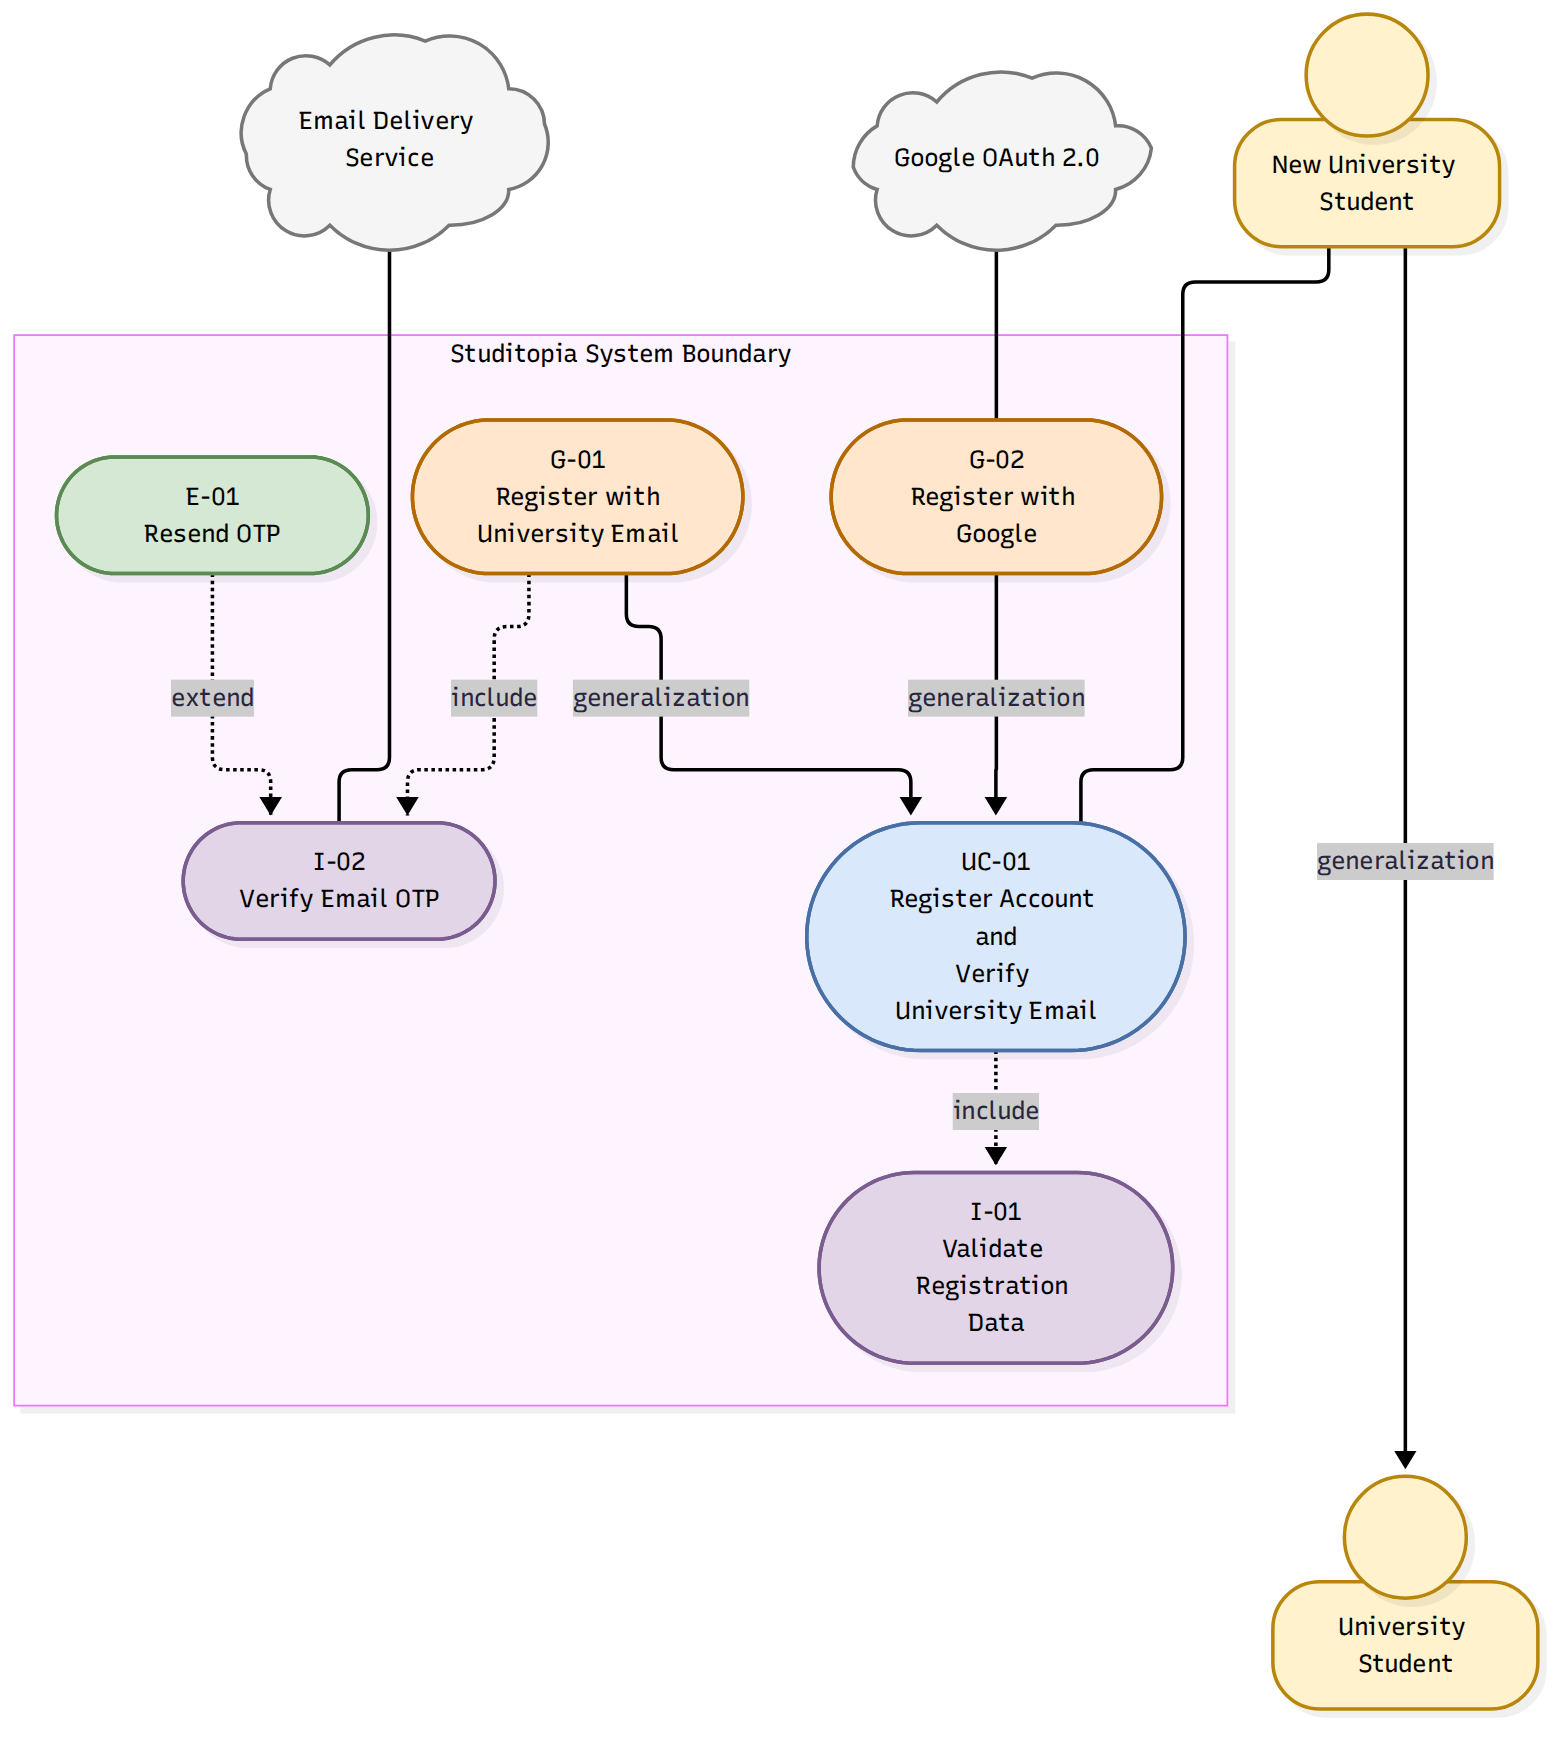
\includegraphics[width=0.85\textwidth,height=0.75\textheight,keepaspectratio]{figures/UC-01.png}
\end{center}
\par\medskip
\textbf{Diagram notation.} Person shape = human actor; cloud = supporting system; blue = selected base use case; purple = included; green = extending; orange = specialized; solid line = association; dashed arrow = include or extend; labelled solid arrow = generalization.
\par\medskip
\hypertarget{sec:1-4-flow-of-events}{}
\addcontentsline{toc}{subsection}{1.4 Flow of Events}
\subsection*{1.4 Flow of Events}
\par\medskip
\hypertarget{sec:1-4-1-basic-flow}{}
\addcontentsline{toc}{subsubsection}{1.4.1 Basic Flow}
\subsubsection*{1.4.1 Basic Flow}
\par\medskip
\begin{enumerate}
\item The user opens the registration page and selects \textbf{Register}.
\item The system displays Display Name, Username, Email, Password, Confirm Password, CAPTCHA, and a \textbf{Continue with Google} option.
\item The user enters the required details and completes the CAPTCHA.
\item The frontend validates that all required fields are present, the email format is valid, the username contains only alphanumeric characters, and the password satisfies the password policy.
\item The frontend verifies that Confirm Password matches Password.
\item The user submits the registration form.
\item The backend validates the submitted data, checks that the email and username are unique, and verifies that the email domain belongs to a supported university or faculty when university-email registration is used.
\item The backend stores a pending account with a securely hashed password and generates a time-limited OTP.
\item The email delivery service sends the OTP to the registered email address, and the system redirects the user to the OTP verification page.
\item The user enters the 6-digit OTP and submits it.
\item The backend verifies that the OTP is valid, unexpired, unused, and correctly formatted.
\item The system activates the account, updates the email-verification status, and authorizes access to Preference Settings.
\item The user completes or updates learning preferences and continues to the Home page.
\end{enumerate}
\par\medskip
\hypertarget{sec:1-4-2-alternative-flows}{}
\addcontentsline{toc}{subsubsection}{1.4.2 Alternative Flows}
\subsubsection*{1.4.2 Alternative Flows}
\par\medskip
Unless otherwise stated, an alternative flow resumes at the next step of the basic flow.
\par\medskip
\hypertarget{sec:a1-google-registration}{}
\paragraph*{A1. Google registration}
\par\medskip
At basic flow step 2, the user selects \textbf{Continue with Google}. The system initiates Google OAuth, validates the authentication response, and creates or associates an account when registration requirements are satisfied. The user then continues to the appropriate next screen, normally Preference Settings.
\par\medskip
\hypertarget{sec:a2-invalid-client-side-input}{}
\paragraph*{A2. Invalid client-side input}
\par\medskip
At basic flow step 4 or 5, validation fails. The system displays field-level errors, keeps the entered values where appropriate, and does not submit the request until the errors are corrected.
\par\medskip
\hypertarget{sec:a3-duplicate-email-or-username}{}
\paragraph*{A3. Duplicate email or username}
\par\medskip
At basic flow step 7, the backend reports that the email or username is already registered. The system displays a clear error and offers navigation to Login or Password Recovery.
\par\medskip
\hypertarget{sec:a4-captcha-verification-failure}{}
\paragraph*{A4. CAPTCHA verification failure}
\par\medskip
At basic flow step 7, CAPTCHA verification fails. The system rejects the request, shows an error, and allows the user to retry.
\par\medskip
\hypertarget{sec:a5-resend-otp}{}
\paragraph*{A5. Resend OTP}
\par\medskip
At basic flow step 10, the user requests a new OTP. The system generates a new 6-digit OTP, invalidates the previous OTP, sends the new code, and restarts the 5-minute expiry period.
\par\medskip
\hypertarget{sec:a6-user-cancels-registration}{}
\paragraph*{A6. User cancels registration}
\par\medskip
The user leaves the registration flow before activation. No active account is available, and the pending verification data remains subject to the system's expiry and cleanup policy.
\par\medskip
\hypertarget{sec:e1-otp-invalid-expired-or-already-used}{}
\paragraph*{E1. OTP invalid, expired, or already used}
\par\medskip
The system rejects the OTP, displays an appropriate message, and keeps the account unverified. The user may request a new OTP.
\par\medskip
\hypertarget{sec:e2-otp-email-delivery-failure}{}
\paragraph*{E2. OTP email delivery failure}
\par\medskip
The account remains unverified and protected features remain unavailable. The system informs the user and allows another OTP request when permitted.
\par\medskip
\hypertarget{sec:e3-google-authentication-fails-or-is-cancelled}{}
\paragraph*{E3. Google authentication fails or is cancelled}
\par\medskip
No account is created or changed by the failed attempt. The system displays an error and allows the user to retry or use manual registration.
\par\medskip
\hypertarget{sec:e4-database-failure-during-account-creation}{}
\paragraph*{E4. Database failure during account creation}
\par\medskip
The registration transaction is rolled back, a generic error is shown, and the user can retry without creating a partial or duplicate account.
\par\medskip
\hypertarget{sec:e5-unverified-account-attempts-protected-access}{}
\paragraph*{E5. Unverified account attempts protected access}
\par\medskip
The backend denies access to protected features until email verification succeeds.
\par\medskip
\hypertarget{sec:1-4-3-business-rules}{}
\addcontentsline{toc}{subsubsection}{1.4.3 Business Rules}
\subsubsection*{1.4.3 Business Rules}
\par\medskip
\begin{enumerate}
\item Display Name, Username, Email, Password, and Confirm Password are required.
\item A username must be unique and contain only alphanumeric characters.
\item An email address must be unique and valid; university-email registration requires a supported university or faculty domain.
\item A password must contain at least 8 characters, including at least one lowercase letter, one uppercase letter, one number, and one special character.
\item Passwords and Confirm Password fields are hidden by default and support a visibility toggle.
\item The OTP is a 6-digit numeric code, expires after 5 minutes, is single-use, and is invalidated when a new OTP is generated.
\item An account cannot access protected application features before successful email verification.
\item The password is persisted only as a secure one-way hash.
\end{enumerate}
\par\medskip
\hypertarget{sec:1-5-special-requirements}{}
\addcontentsline{toc}{subsection}{1.5 Special Requirements}
\subsection*{1.5 Special Requirements}
\par\medskip
\begingroup
\small
\renewcommand{\baselinestretch}{1.0}\selectfont
\renewcommand{\arraystretch}{1.15}
\setlength{\tabcolsep}{6pt}
\begin{longtable}{|>{\raggedright\arraybackslash}p{0.22\textwidth}|>{\raggedright\arraybackslash}p{0.73\textwidth}|}
\hline
\textbf{ID} & \textbf{Requirement} \\ \hline
\endhead
NFR-SEC-2 & User credentials must be stored using one-way password hashing with a secure hashing algorithm. \\ \hline
NFR-SEC-3 & Sensitive communication must be encrypted using TLS 1.2 or higher. \\ \hline
NFR-SEC-8 & The system must protect against common web security vulnerabilities, including SQL injection, XSS, and CSRF. \\ \hline
NFR-USE-1 & A new university student must be able to complete registration within 5 minutes without external assistance. \\ \hline
Design constraint & The OTP is 6 digits, single-use, and expires after 5 minutes. The password policy and field visibility rules must be enforced by both frontend and backend validation. \\ \hline
\end{longtable}
\endgroup
\par\medskip
\hypertarget{sec:1-6-preconditions}{}
\addcontentsline{toc}{subsection}{1.6 Preconditions}
\subsection*{1.6 Preconditions}
\par\medskip
\begin{enumerate}
\item The user does not have an active authenticated session.
\item The supported university and faculty email-domain catalog is available for university-email registration.
\item The email delivery service is available for the standard registration path.
\item Google OAuth 2.0 is configured for the optional Google registration path.
\end{enumerate}
\par\medskip
\hypertarget{sec:1-7-postconditions}{}
\addcontentsline{toc}{subsection}{1.7 Postconditions}
\subsection*{1.7 Postconditions}
\par\medskip
\begin{enumerate}
\item \textbf{Success:} A user record exists with a unique username and email address, and the account is activated and email-verified.
\item \textbf{Success:} The user's password is stored only as a secure one-way hash; Google registration associates the authenticated Google identity with the account.
\item \textbf{Success:} The user is authorized to continue to Preference Settings and then the Home page.
\item \textbf{Failure:} No active account is created, and the user receives an error message that allows correction and retry.
\item \textbf{Failure:} An unverified account, if created, cannot access protected application features.
\end{enumerate}
\par\medskip
\hypertarget{sec:1-8-extension-points}{}
\addcontentsline{toc}{subsection}{1.8 Extension Points}
\subsection*{1.8 Extension Points}
\par\medskip
\begingroup
\small
\renewcommand{\baselinestretch}{1.0}\selectfont
\renewcommand{\arraystretch}{1.15}
\setlength{\tabcolsep}{6pt}
\begin{longtable}{|>{\raggedright\arraybackslash}p{0.35\textwidth}|>{\raggedright\arraybackslash}p{0.6\textwidth}|}
\hline
\textbf{Extension Point} & \textbf{Location in Flow of Events} \\ \hline
\endhead
Google registration & Basic flow step 2; alternative flow A1 \\ \hline
Client-side validation recovery & Basic flow steps 4-5; alternative flow A2 \\ \hline
Duplicate-account handling & Basic flow step 7; alternative flow A3 \\ \hline
CAPTCHA retry & Basic flow step 7; alternative flow A4 \\ \hline
OTP resend & Basic flow step 10; alternative flow A5 and exceptions E1-E2 \\ \hline
Registration cancellation & Any step before activation; alternative flow A6 \\ \hline
Unverified-access recovery & Protected-feature access; exception E5 \\ \hline
\end{longtable}
\endgroup
\par\medskip
\par\noindent\rule{\linewidth}{0.4pt}\par\medskip
\hypertarget{sec:2-uc-02-log-in}{}
\hypertarget{2-uc-02-log-in}{}
\addcontentsline{toc}{section}{2. UC-02 Log In}
\section*{2. UC-02 Log In}
\par\medskip
\hypertarget{sec:2-1-use-case-name}{}
\addcontentsline{toc}{subsection}{2.1 Use-Case Name}
\subsection*{2.1 Use-Case Name}
\par\medskip
\texttt{UC-02 Log In}
\par\medskip
\hypertarget{sec:2-2-brief-description}{}
\addcontentsline{toc}{subsection}{2.2 Brief Description}
\subsection*{2.2 Brief Description}
\par\medskip
A registered university student authenticates and regains access to their profile, university forum, posts, and learning activities. Login supports a registered username or university email with a password, and an optional Google OAuth path.
\par\medskip
\begingroup
\small
\renewcommand{\baselinestretch}{1.0}\selectfont
\renewcommand{\arraystretch}{1.15}
\setlength{\tabcolsep}{6pt}
\begin{longtable}{|>{\raggedright\arraybackslash}p{0.28\textwidth}|>{\raggedright\arraybackslash}p{0.67\textwidth}|}
\hline
\textbf{Field} & \textbf{Value} \\ \hline
\endhead
Use Case ID & UC-02 \\ \hline
Primary Actor & Registered University Student \\ \hline
Supporting Actors & Google OAuth 2.0 \\ \hline
Feature Group & Authentication \\ \hline
Priority & High \\ \hline
Related User Stories & US-02 \\ \hline
Related Requirements & FR-02.1 to FR-02.5; FR-04.1 to FR-04.4; NFR-SEC-1, NFR-SEC-3, NFR-SEC-6, NFR-SEC-7, NFR-SEC-8 \\ \hline
\end{longtable}
\endgroup
\par\medskip
\hypertarget{sec:2-3-use-case-diagram}{}
\addcontentsline{toc}{subsection}{2.3 Use Case Diagram}
\subsection*{2.3 Use Case Diagram}
\par\medskip
\begin{center}
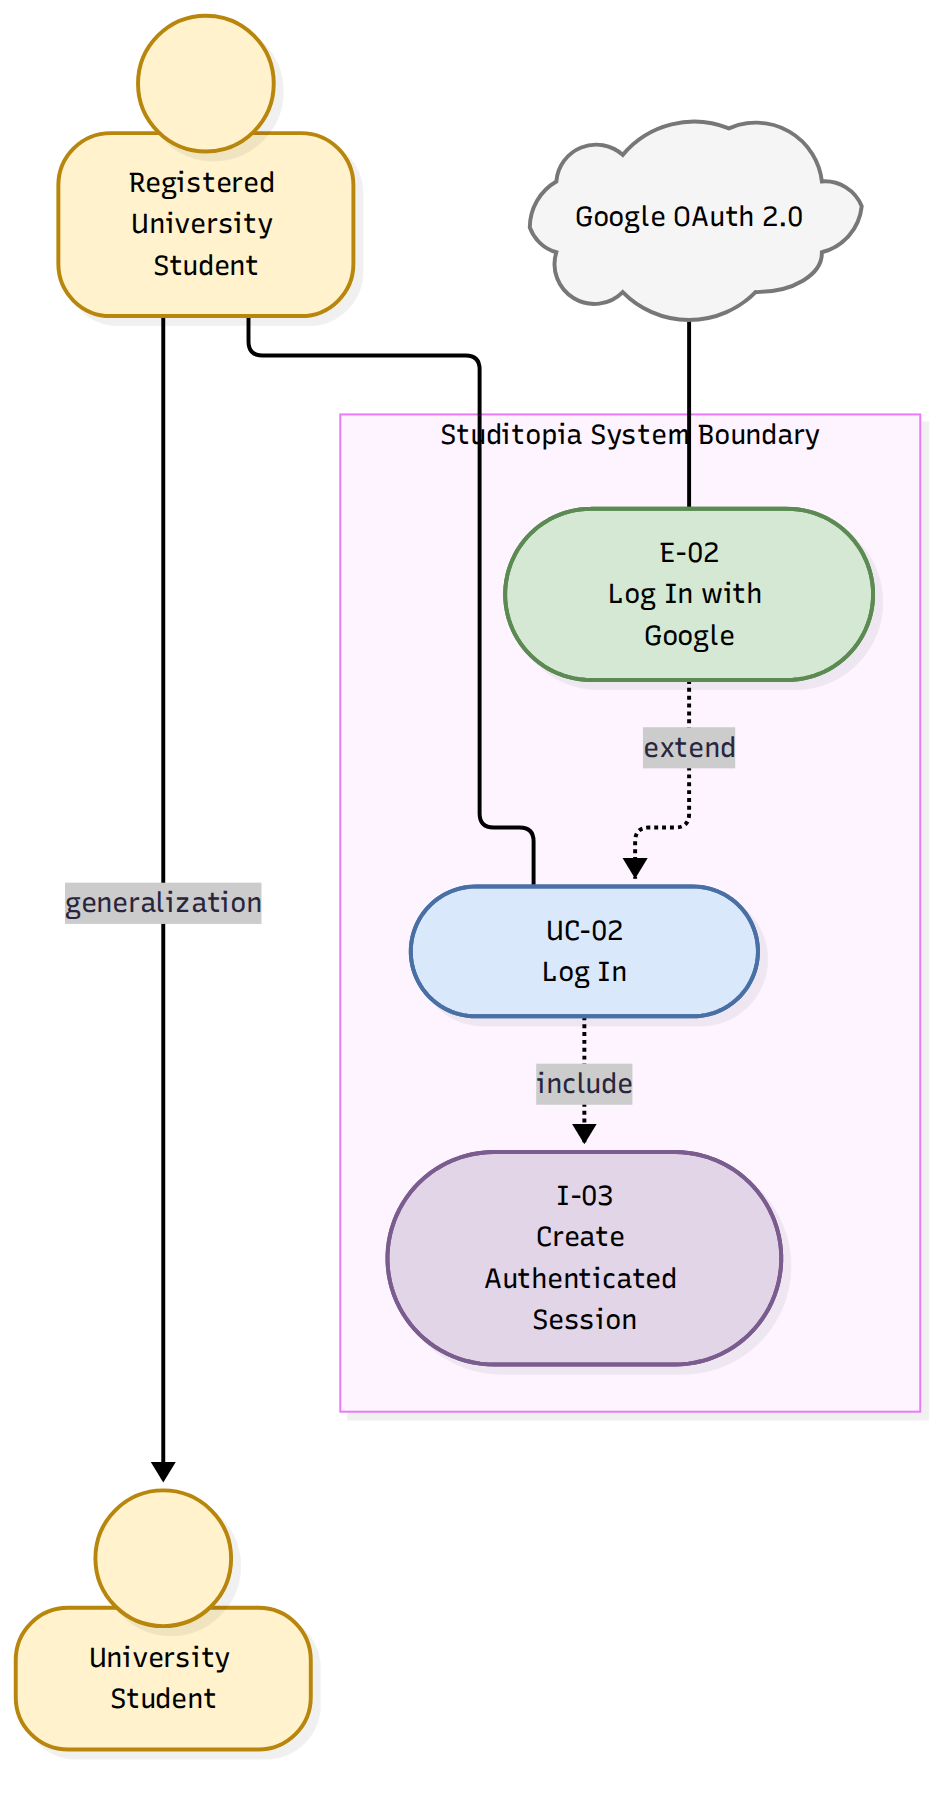
\includegraphics[width=0.85\textwidth,height=0.75\textheight,keepaspectratio]{figures/UC-02.png}
\end{center}
\par\medskip
\textbf{Diagram notation.} Person shape = human actor; cloud = supporting system; blue = selected base use case; purple = included; green = extending; solid line = association; dashed arrow = include or extend; labelled solid arrow = generalization.
\par\medskip
\hypertarget{sec:2-4-flow-of-events}{}
\addcontentsline{toc}{subsection}{2.4 Flow of Events}
\subsection*{2.4 Flow of Events}
\par\medskip
\hypertarget{sec:2-4-1-basic-flow}{}
\addcontentsline{toc}{subsubsection}{2.4.1 Basic Flow}
\subsubsection*{2.4.1 Basic Flow}
\par\medskip
\begin{enumerate}
\item The student opens the login page.
\item The system displays the username-or-email field, password field, CAPTCHA, \textbf{Remember Me} option where supported, \textbf{Forget Password}, \textbf{Register}, and \textbf{Continue with Google} options.
\item The student enters a registered username or university email address and password, then completes the CAPTCHA.
\item The frontend performs basic input validation and submits the login request.
\item The backend verifies the CAPTCHA, credentials, account activation status, and any account restrictions.
\item The backend creates an authenticated session and returns the access result.
\item The frontend stores the session according to the \textbf{Remember Me} choice, loads the student's profile and forum context, and redirects to Home or the intended protected page.
\item The system displays the Home page with the Forum entry and the student's university forum as the default context.
\end{enumerate}
\par\medskip
\hypertarget{sec:2-4-2-alternative-flows}{}
\addcontentsline{toc}{subsubsection}{2.4.2 Alternative Flows}
\subsubsection*{2.4.2 Alternative Flows}
\par\medskip
Unless otherwise stated, an alternative flow resumes at the next step of the basic flow.
\par\medskip
\hypertarget{sec:a1-google-login}{}
\paragraph*{A1. Google login}
\par\medskip
At basic flow step 2, the student selects \textbf{Continue with Google}. The system completes Google OAuth, validates the response, and either creates the authenticated session or displays an appropriate error.
\par\medskip
\hypertarget{sec:a2-remember-me-selected}{}
\paragraph*{A2. Remember Me selected}
\par\medskip
At basic flow step 7, the system maintains the session across browser restarts according to the selected option and the platform session policy.
\par\medskip
\hypertarget{sec:a3-intended-page-available}{}
\paragraph*{A3. Intended page available}
\par\medskip
If the student was redirected from a protected page, the system returns the student to that page after successful authentication instead of Home.
\par\medskip
\hypertarget{sec:a4-unverified-account}{}
\paragraph*{A4. Unverified account}
\par\medskip
If the backend finds that the account is not verified, login is denied and the student is directed to complete OTP verification.
\par\medskip
\hypertarget{sec:e1-invalid-credentials}{}
\paragraph*{E1. Invalid credentials}
\par\medskip
The system displays a clear error without revealing whether the username, email, or password was incorrect.
\par\medskip
\hypertarget{sec:e2-captcha-failure}{}
\paragraph*{E2. CAPTCHA failure}
\par\medskip
The system rejects the request, displays an error, and allows the student to retry.
\par\medskip
\hypertarget{sec:e3-unavailable-or-restricted-account}{}
\paragraph*{E3. Unavailable or restricted account}
\par\medskip
The system denies authentication and displays an appropriate message without exposing sensitive account details.
\par\medskip
\hypertarget{sec:e4-authentication-service-failure}{}
\paragraph*{E4. Authentication service failure}
\par\medskip
No session is created. The system displays a temporary error and allows the student to retry.
\par\medskip
\hypertarget{sec:e5-session-expires-while-accessing-a-protected-page}{}
\paragraph*{E5. Session expires while accessing a protected page}
\par\medskip
The system denies access, informs the student that the session expired, and requires login again.
\par\medskip
\hypertarget{sec:2-4-3-business-rules}{}
\addcontentsline{toc}{subsubsection}{2.4.3 Business Rules}
\subsubsection*{2.4.3 Business Rules}
\par\medskip
\begin{enumerate}
\item Login is accepted with either a registered username or a registered university email address.
\item Invalid-credential messages must not reveal which credential field was incorrect.
\item CAPTCHA must be successfully verified before login processing.
\item Google login is an optional authentication path for registered users.
\item Protected pages and APIs require a valid authenticated session.
\item After successful login, the student's profile, forum, posts, and learning activities are accessible according to their permissions.
\item The session is subject to the platform's inactivity-expiry policy.
\end{enumerate}
\par\medskip
\hypertarget{sec:2-5-special-requirements}{}
\addcontentsline{toc}{subsection}{2.5 Special Requirements}
\subsection*{2.5 Special Requirements}
\par\medskip
\begingroup
\small
\renewcommand{\baselinestretch}{1.0}\selectfont
\renewcommand{\arraystretch}{1.15}
\setlength{\tabcolsep}{6pt}
\begin{longtable}{|>{\raggedright\arraybackslash}p{0.22\textwidth}|>{\raggedright\arraybackslash}p{0.73\textwidth}|}
\hline
\textbf{ID} & \textbf{Requirement} \\ \hline
\endhead
NFR-SEC-1 & Authentication is required before accessing protected user resources. \\ \hline
NFR-SEC-3 & Sensitive communication must be encrypted using TLS 1.2 or higher. \\ \hline
NFR-SEC-6 & Server-side authorization checks must prevent unauthorized access. \\ \hline
NFR-SEC-7 & Inactive authentication sessions must expire automatically after 30 minutes. \\ \hline
NFR-SEC-8 & The system must protect against SQL injection, XSS, CSRF, and other common web vulnerabilities. \\ \hline
\end{longtable}
\endgroup
\par\medskip
\hypertarget{sec:2-6-preconditions}{}
\addcontentsline{toc}{subsection}{2.6 Preconditions}
\subsection*{2.6 Preconditions}
\par\medskip
\begin{enumerate}
\item The student has a registered and activated account.
\item The student is not already authenticated, or chooses to start a new authenticated session.
\item The authentication service and, when used, Google OAuth 2.0 are available.
\end{enumerate}
\par\medskip
\hypertarget{sec:2-7-postconditions}{}
\addcontentsline{toc}{subsection}{2.7 Postconditions}
\subsection*{2.7 Postconditions}
\par\medskip
\begin{enumerate}
\item \textbf{Success:} A valid authenticated session is created and the student reaches the Home page or the originally requested protected page.
\item \textbf{Success:} The student's default university forum context is available after login.
\item \textbf{Failure:} No authenticated session is created, and the student remains on the login page with a non-disclosing error message.
\end{enumerate}
\par\medskip
\hypertarget{sec:2-8-extension-points}{}
\addcontentsline{toc}{subsection}{2.8 Extension Points}
\subsection*{2.8 Extension Points}
\par\medskip
\begingroup
\small
\renewcommand{\baselinestretch}{1.0}\selectfont
\renewcommand{\arraystretch}{1.15}
\setlength{\tabcolsep}{6pt}
\begin{longtable}{|>{\raggedright\arraybackslash}p{0.35\textwidth}|>{\raggedright\arraybackslash}p{0.6\textwidth}|}
\hline
\textbf{Extension Point} & \textbf{Location in Flow of Events} \\ \hline
\endhead
Google login & Basic flow step 2; alternative flow A1 \\ \hline
Remember Me & Basic flow step 7; alternative flow A2 \\ \hline
Return to intended page & Basic flow step 8; alternative flow A3 \\ \hline
Unverified-account recovery & Basic flow step 5; alternative flow A4 \\ \hline
Session expiry & Protected-page access; exception E5 \\ \hline
\end{longtable}
\endgroup
\par\medskip
\par\noindent\rule{\linewidth}{0.4pt}\par\medskip
\hypertarget{sec:3-uc-03-browse-and-search-the-university-forum}{}
\hypertarget{3-uc-03-browse-and-search-the-university-forum}{}
\addcontentsline{toc}{section}{3. UC-03 Browse and Search the University Forum}
\section*{3. UC-03 Browse and Search the University Forum}
\par\medskip
\hypertarget{sec:3-1-use-case-name}{}
\addcontentsline{toc}{subsection}{3.1 Use-Case Name}
\subsection*{3.1 Use-Case Name}
\par\medskip
\texttt{UC-03 Browse and Search the University Forum}
\par\medskip
\hypertarget{sec:3-2-brief-description}{}
\addcontentsline{toc}{subsection}{3.2 Brief Description}
\subsection*{3.2 Brief Description}
\par\medskip
A student discovers relevant university, major, and course discussions, searches for academic content, and opens a post to read its full details. The forum is the primary collaboration feature of Studitopia.
\par\medskip
\begingroup
\small
\renewcommand{\baselinestretch}{1.0}\selectfont
\renewcommand{\arraystretch}{1.15}
\setlength{\tabcolsep}{6pt}
\begin{longtable}{|>{\raggedright\arraybackslash}p{0.28\textwidth}|>{\raggedright\arraybackslash}p{0.67\textwidth}|}
\hline
\textbf{Field} & \textbf{Value} \\ \hline
\endhead
Use Case ID & UC-03 \\ \hline
Primary Actor & University Student \\ \hline
Supporting Actors & None \\ \hline
Feature Group & Forum (Primary) \\ \hline
Priority & High \\ \hline
Related User Stories & US-11, US-12, US-13, US-17, US-23 \\ \hline
Related Requirements & FR-11.1 to FR-11.4; FR-12.1 to FR-12.6; FR-13.1 to FR-13.5; FR-17.1 to FR-17.5; FR-23.1 to FR-23.5; NFR-PERF-2, NFR-PERF-3, NFR-PERF-5, NFR-SEC-4, NFR-SEC-6, NFR-PRIV-7, NFR-USE-3 \\ \hline
\end{longtable}
\endgroup
\par\medskip
\hypertarget{sec:3-3-use-case-diagram}{}
\addcontentsline{toc}{subsection}{3.3 Use Case Diagram}
\subsection*{3.3 Use Case Diagram}
\par\medskip
\begin{center}
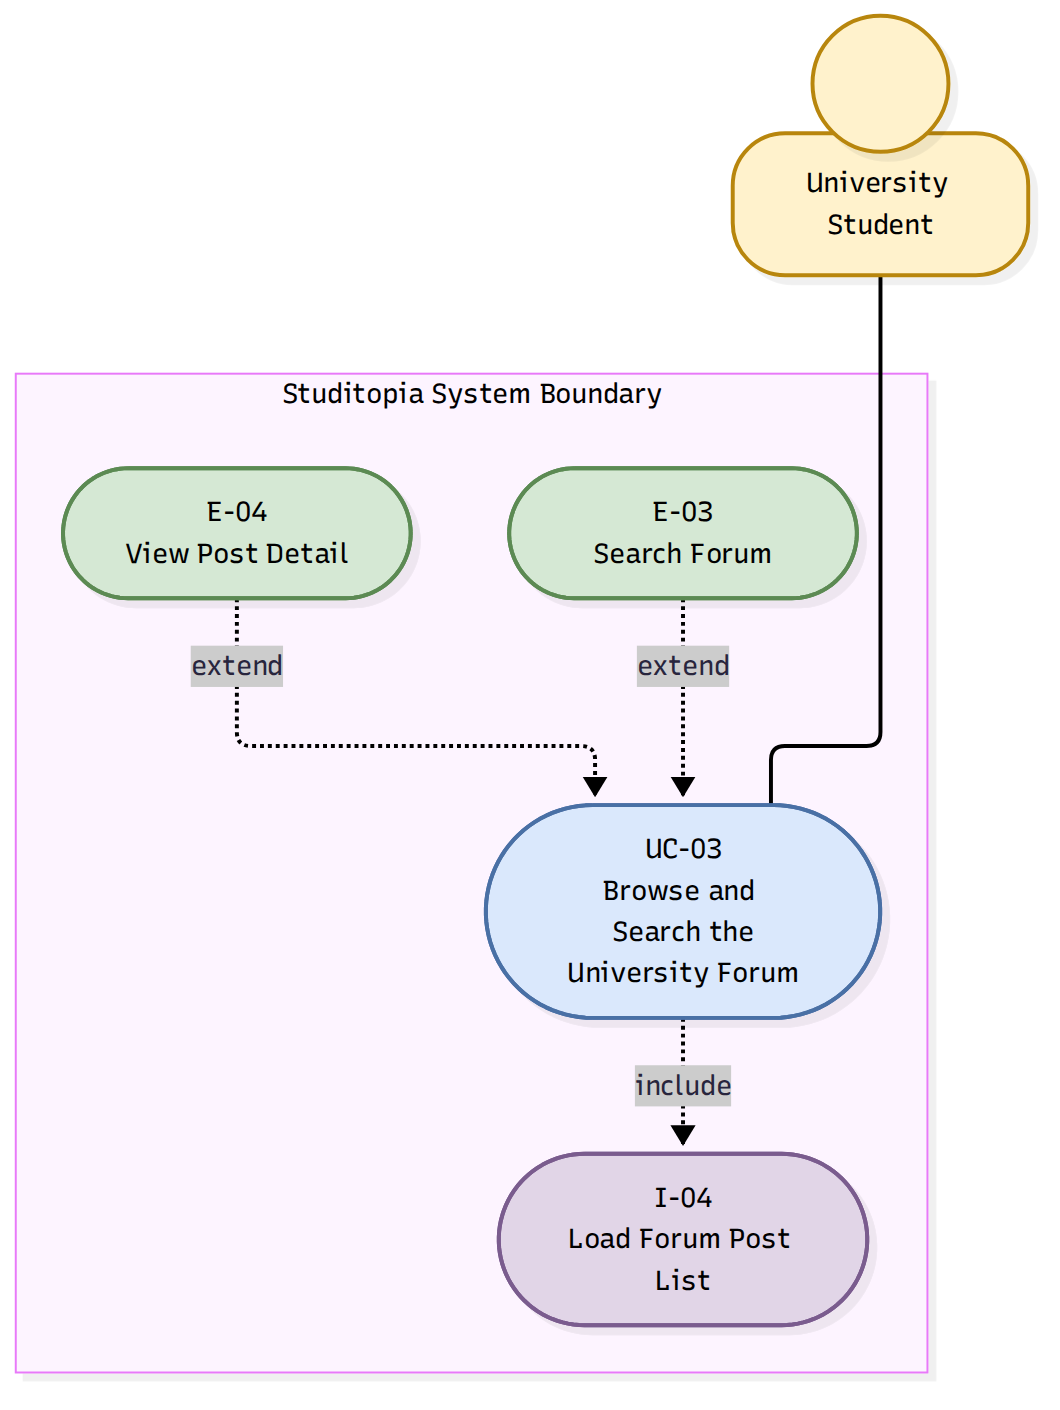
\includegraphics[width=0.85\textwidth,height=0.75\textheight,keepaspectratio]{figures/UC-03.png}
\end{center}
\par\medskip
\textbf{Diagram notation.} Person shape = human actor; blue = selected base use case; purple = included; green = extending; solid line = association; dashed arrow = include or extend.
\par\medskip
\hypertarget{sec:3-4-flow-of-events}{}
\addcontentsline{toc}{subsection}{3.4 Flow of Events}
\subsection*{3.4 Flow of Events}
\par\medskip
\hypertarget{sec:3-4-1-basic-flow}{}
\addcontentsline{toc}{subsubsection}{3.4.1 Basic Flow}
\subsubsection*{3.4.1 Basic Flow}
\par\medskip
\begin{enumerate}
\item The student selects \textbf{Forum} from the main navigation.
\item The system opens the student's default university forum and displays the Forum entry, forum hierarchy, and post list.
\item The student selects a university; the system displays the majors offered by that university.
\item The student selects a major; the system displays the courses associated with that major.
\item The student selects a course; the system displays the course forum and its posts.
\item The system shows each post summary with title, author, post type, timestamp, vote score, comment count, and solved status.
\item The student optionally applies filters such as My Post, area, university, major, course, tags, and post type, and selects a sorting order such as newest, top trending, most voted, or most discussed.
\item The student optionally enters a keyword and searches by tag, title, content, author, university, major, or course.
\item The system ranks matching results by relevance and engagement and displays the filtered result set.
\item The student opens a post from the list or search results.
\item The system displays the full post content, author, post type, forum context, timestamp, vote score, tags, comments, answers, true response, attachments, and functional tools when present.
\item The system displays only the actions permitted for the student, such as vote, comment, save, report, or mark true response.
\end{enumerate}
\par\medskip
\hypertarget{sec:3-4-2-alternative-flows}{}
\addcontentsline{toc}{subsubsection}{3.4.2 Alternative Flows}
\subsubsection*{3.4.2 Alternative Flows}
\par\medskip
Unless otherwise stated, an alternative flow resumes at the next step of the basic flow.
\par\medskip
\hypertarget{sec:a1-browse-another-university}{}
\paragraph*{A1. Browse another university}
\par\medskip
At basic flow step 3, the student selects another university forum when permitted. The system applies that university as the active browsing context and shows only content relevant to that context.
\par\medskip
\hypertarget{sec:a2-change-forum-context}{}
\paragraph*{A2. Change forum context}
\par\medskip
The student switches directly between university, major, and course levels. The system updates the post list to match the selected level.
\par\medskip
\hypertarget{sec:a3-no-posts-match}{}
\paragraph*{A3. No posts match}
\par\medskip
At basic flow step 9 or 10, no posts match the filters or search query. The system displays an empty state and offers to clear filters or change the search terms.
\par\medskip
\hypertarget{sec:a4-search-without-a-keyword}{}
\paragraph*{A4. Search without a keyword}
\par\medskip
The student applies only filters. The system returns results based on the selected forum context and filters.
\par\medskip
\hypertarget{sec:a5-return-to-a-previous-context}{}
\paragraph*{A5. Return to a previous context}
\par\medskip
The student navigates back; the system restores the previous forum level and result state where supported.
\par\medskip
\hypertarget{sec:e1-forum-content-cannot-be-loaded}{}
\paragraph*{E1. Forum content cannot be loaded}
\par\medskip
The system displays an error state and a retry option without showing partial or stale restricted content.
\par\medskip
\hypertarget{sec:e2-selected-post-is-unavailable-or-deleted}{}
\paragraph*{E2. Selected post is unavailable or deleted}
\par\medskip
The system informs the student that the post is no longer available and returns them to the post list.
\par\medskip
\hypertarget{sec:e3-access-is-not-permitted}{}
\paragraph*{E3. Access is not permitted}
\par\medskip
The system denies access to private or restricted content and explains that the student lacks permission.
\par\medskip
\hypertarget{sec:e4-invalid-search-or-filter-combination}{}
\paragraph*{E4. Invalid search or filter combination}
\par\medskip
The system displays validation feedback and preserves the usable parts of the query.
\par\medskip
\hypertarget{sec:3-4-3-business-rules}{}
\addcontentsline{toc}{subsubsection}{3.4.3 Business Rules}
\subsubsection*{3.4.3 Business Rules}
\par\medskip
\begin{enumerate}
\item Forum content is organized by University, then Major, then Course.
\item After login, the student's own university is the default forum context.
\item Each forum level must display only posts and materials relevant to that level.
\item Post summaries must include title, author, post type, timestamp, vote score, comment count, and solved status.
\item Search supports tags, title, content, author, university, major, and course.
\item Search results are ranked by relevance and engagement and can be filtered by post type, solved status, and time range.
\item Post detail must show the full content, metadata, discussion, marked true response, attachments, and functional tools when present.
\item Available post actions are determined by the student's permissions.
\item Privacy and forum-access rules apply consistently to post lists, post details, and search results.
\end{enumerate}
\par\medskip
\hypertarget{sec:3-5-special-requirements}{}
\addcontentsline{toc}{subsection}{3.5 Special Requirements}
\subsection*{3.5 Special Requirements}
\par\medskip
\begingroup
\small
\renewcommand{\baselinestretch}{1.0}\selectfont
\renewcommand{\arraystretch}{1.15}
\setlength{\tabcolsep}{6pt}
\begin{longtable}{|>{\raggedright\arraybackslash}p{0.22\textwidth}|>{\raggedright\arraybackslash}p{0.73\textwidth}|}
\hline
\textbf{ID} & \textbf{Requirement} \\ \hline
\endhead
NFR-PERF-2 & A forum post list must load within 2 seconds under normal operating conditions. \\ \hline
NFR-PERF-3 & A post detail page and its comments must display within 2 seconds. \\ \hline
NFR-PERF-5 & Forum search results must return within 2 seconds for common queries. \\ \hline
NFR-SEC-4 & Private forum content and private-group content must be restricted to authorized users only. \\ \hline
NFR-SEC-6 & Server-side authorization checks must prevent unauthorized access. \\ \hline
NFR-PRIV-7 & Privacy settings must apply consistently to forum posts, comments, member lists, and search results. \\ \hline
NFR-USE-3 & Navigation and interaction patterns must remain consistent across university, major, and course forums. \\ \hline
\end{longtable}
\endgroup
\par\medskip
\hypertarget{sec:3-6-preconditions}{}
\addcontentsline{toc}{subsection}{3.6 Preconditions}
\subsection*{3.6 Preconditions}
\par\medskip
\begin{enumerate}
\item The student is authenticated with an active session.
\item University, major, course, and forum data are available.
\item The student has permission to view the selected forum content.
\end{enumerate}
\par\medskip
\hypertarget{sec:3-7-postconditions}{}
\addcontentsline{toc}{subsection}{3.7 Postconditions}
\subsection*{3.7 Postconditions}
\par\medskip
\begin{enumerate}
\item \textbf{Success:} The selected forum level and a relevant post list are displayed.
\item \textbf{Success:} Search and filters return ranked results, or a clear empty state is shown when nothing matches.
\item \textbf{Success:} The student can open a post and read its full content, metadata, discussion, attachments, and permitted actions.
\item \textbf{Failure:} The system displays an error or permission message without exposing restricted content.
\end{enumerate}
\par\medskip
\hypertarget{sec:3-8-extension-points}{}
\addcontentsline{toc}{subsection}{3.8 Extension Points}
\subsection*{3.8 Extension Points}
\par\medskip
\begingroup
\small
\renewcommand{\baselinestretch}{1.0}\selectfont
\renewcommand{\arraystretch}{1.15}
\setlength{\tabcolsep}{6pt}
\begin{longtable}{|>{\raggedright\arraybackslash}p{0.35\textwidth}|>{\raggedright\arraybackslash}p{0.6\textwidth}|}
\hline
\textbf{Extension Point} & \textbf{Location in Flow of Events} \\ \hline
\endhead
Change browsing context & Basic flow steps 3-5; alternatives A1-A2 \\ \hline
Apply filters & Basic flow step 7; alternative A4 \\ \hline
Search forum & Basic flow step 8; alternative A3 and exception E4 \\ \hline
View post detail & Basic flow step 10; exception E2 \\ \hline
Empty-result recovery & Basic flow step 9; alternative A3 \\ \hline
Restricted-content handling & Access check; exception E3 \\ \hline
\end{longtable}
\endgroup
\par\medskip
\par\noindent\rule{\linewidth}{0.4pt}\par\medskip
\hypertarget{sec:4-uc-04-create-discussion-post}{}
\hypertarget{4-uc-04-create-discussion-post}{}
\addcontentsline{toc}{section}{4. UC-04 Create Discussion Post}
\section*{4. UC-04 Create Discussion Post}
\par\medskip
\hypertarget{sec:4-1-use-case-name}{}
\addcontentsline{toc}{subsection}{4.1 Use-Case Name}
\subsection*{4.1 Use-Case Name}
\par\medskip
\texttt{UC-04 Create Discussion Post}
\par\medskip
\hypertarget{sec:4-2-brief-description}{}
\addcontentsline{toc}{subsection}{4.2 Brief Description}
\subsection*{4.2 Brief Description}
\par\medskip
A student publishes an academic question or general discussion in the selected university, major, and course forum. The post supports text, optional LaTeX, optional images, and tags.
\par\medskip
\begingroup
\small
\renewcommand{\baselinestretch}{1.0}\selectfont
\renewcommand{\arraystretch}{1.15}
\setlength{\tabcolsep}{6pt}
\begin{longtable}{|>{\raggedright\arraybackslash}p{0.28\textwidth}|>{\raggedright\arraybackslash}p{0.67\textwidth}|}
\hline
\textbf{Field} & \textbf{Value} \\ \hline
\endhead
Use Case ID & UC-04 \\ \hline
Primary Actor & University Student \\ \hline
Supporting Actors & None \\ \hline
Feature Group & Forum (Primary) \\ \hline
Priority & High \\ \hline
Related User Stories & US-14 \\ \hline
Related Requirements & FR-14.1 to FR-14.6; FR-17.1 to FR-17.5; FR-19.1 to FR-19.5; FR-20.1 to FR-20.5; NFR-PERF-4, NFR-SEC-8, NFR-SEC-9 \\ \hline
\end{longtable}
\endgroup
\par\medskip
\hypertarget{sec:4-3-use-case-diagram}{}
\addcontentsline{toc}{subsection}{4.3 Use Case Diagram}
\subsection*{4.3 Use Case Diagram}
\par\medskip
\begin{center}
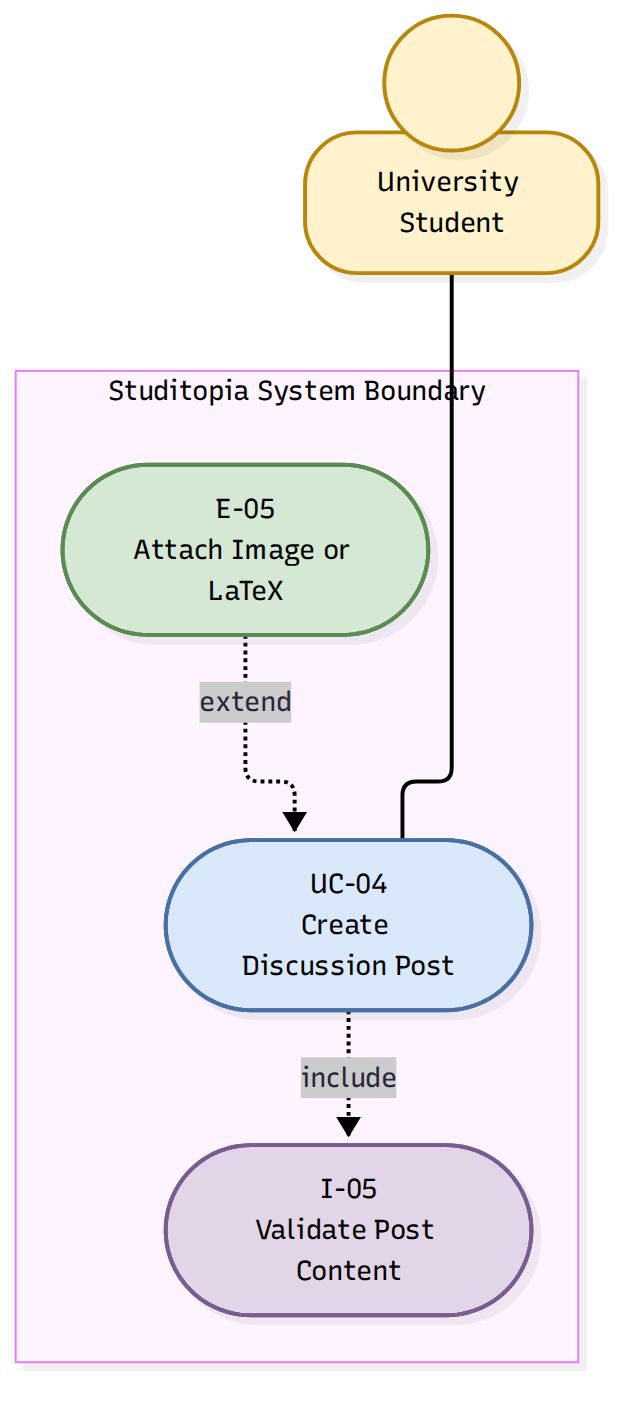
\includegraphics[width=0.85\textwidth,height=0.75\textheight,keepaspectratio]{figures/UC-04.png}
\end{center}
\par\medskip
\textbf{Diagram notation.} Person shape = human actor; blue = selected base use case; purple = included; green = extending; solid line = association; dashed arrow = include or extend.
\par\medskip
\hypertarget{sec:4-4-flow-of-events}{}
\addcontentsline{toc}{subsection}{4.4 Flow of Events}
\subsection*{4.4 Flow of Events}
\par\medskip
\hypertarget{sec:4-4-1-basic-flow}{}
\addcontentsline{toc}{subsubsection}{4.4.1 Basic Flow}
\subsubsection*{4.4.1 Basic Flow}
\par\medskip
\begin{enumerate}
\item The student selects \textbf{Create Post} from the selected forum.
\item The system displays the post-type choices and the discussion post editor.
\item The system shows the active university, major, and course context for the new post.
\item The student enters a title, text content, optional LaTeX, optional images, and tags.
\item The student marks the post as a question or a general discussion.
\item The frontend validates the required content and supported image types or sizes before submission.
\item The student submits the post.
\item The backend verifies authentication, forum access, post permissions, content, and rate limits.
\item The backend stores the post with its author, post type, tags, and university, major, and course associations.
\item The system publishes the post and returns the new post result.
\item The system displays the post in the corresponding forum post list and allows the student to open its detail page.
\end{enumerate}
\par\medskip
\hypertarget{sec:4-4-2-alternative-flows}{}
\addcontentsline{toc}{subsubsection}{4.4.2 Alternative Flows}
\subsubsection*{4.4.2 Alternative Flows}
\par\medskip
Unless otherwise stated, an alternative flow resumes at the next step of the basic flow.
\par\medskip
\hypertarget{sec:a1-general-discussion}{}
\paragraph*{A1. General discussion}
\par\medskip
At basic flow step 5, the student selects \textbf{General Discussion} instead of \textbf{Question}. The publication flow is unchanged, but the post is not treated as a question awaiting a true response.
\par\medskip
\hypertarget{sec:a2-question-post}{}
\paragraph*{A2. Question post}
\par\medskip
At basic flow step 5, the student selects \textbf{Question}. The post becomes eligible for answers and true-response marking after publication.
\par\medskip
\hypertarget{sec:a3-add-or-remove-optional-content}{}
\paragraph*{A3. Add or remove optional content}
\par\medskip
At basic flow step 4, the student adds or removes LaTeX, images, or tags. The editor updates the preview and validation state before submission.
\par\medskip
\hypertarget{sec:a4-cancel-creation}{}
\paragraph*{A4. Cancel creation}
\par\medskip
The student leaves the editor before submitting. No published post is created; any retained draft behavior is subject to the platform's buffering policy.
\par\medskip
\hypertarget{sec:e1-missing-or-invalid-content}{}
\paragraph*{E1. Missing or invalid content}
\par\medskip
The system highlights the invalid fields, keeps the editor open, and does not submit until corrected.
\par\medskip
\hypertarget{sec:e2-unsupported-or-oversized-image}{}
\paragraph*{E2. Unsupported or oversized image}
\par\medskip
The system rejects the image, identifies the constraint, and allows the student to choose another file.
\par\medskip
\hypertarget{sec:e3-forum-access-lost}{}
\paragraph*{E3. Forum access lost}
\par\medskip
If the forum context is no longer valid or the student lacks posting permission, the system rejects publication and explains the reason.
\par\medskip
\hypertarget{sec:e4-rate-limit-reached}{}
\paragraph*{E4. Rate limit reached}
\par\medskip
The system rejects the submission and informs the student to retry later.
\par\medskip
\hypertarget{sec:e5-server-or-database-failure}{}
\paragraph*{E5. Server or database failure}
\par\medskip
No post is published. The system displays a retry option and preserves the student's entered content where supported.
\par\medskip
\hypertarget{sec:4-4-3-business-rules}{}
\addcontentsline{toc}{subsubsection}{4.4.3 Business Rules}
\subsubsection*{4.4.3 Business Rules}
\par\medskip
\begin{enumerate}
\item A discussion post must be associated with the selected university, major, and course.
\item A discussion post supports a title, text content, LaTeX, images, and tags.
\item The author must choose whether the post is a question or a general discussion.
\item Content must pass frontend and backend validation before publication.
\item A published post must appear in the corresponding forum post list.
\item Only authenticated and authorized students may create posts in a forum.
\item Post publication is subject to rate limiting to reduce spam and abuse.
\end{enumerate}
\par\medskip
\hypertarget{sec:4-5-special-requirements}{}
\addcontentsline{toc}{subsection}{4.5 Special Requirements}
\subsection*{4.5 Special Requirements}
\par\medskip
\begingroup
\small
\renewcommand{\baselinestretch}{1.0}\selectfont
\renewcommand{\arraystretch}{1.15}
\setlength{\tabcolsep}{6pt}
\begin{longtable}{|>{\raggedright\arraybackslash}p{0.22\textwidth}|>{\raggedright\arraybackslash}p{0.73\textwidth}|}
\hline
\textbf{ID} & \textbf{Requirement} \\ \hline
\endhead
NFR-PERF-4 & A new post must be reflected in the relevant forum view within 2 seconds. \\ \hline
NFR-SEC-8 & The system must protect against SQL injection, XSS, CSRF, and other common web vulnerabilities. \\ \hline
NFR-SEC-9 & Post creation must be rate-limited to reduce spam and abuse. \\ \hline
Design constraint & The editor must validate required content, supported image types, and image sizes before submission. LaTeX and images are optional. \\ \hline
\end{longtable}
\endgroup
\par\medskip
\hypertarget{sec:4-6-preconditions}{}
\addcontentsline{toc}{subsection}{4.6 Preconditions}
\subsection*{4.6 Preconditions}
\par\medskip
\begin{enumerate}
\item The student is authenticated with an active session.
\item The student has selected a valid university, major, and course forum context.
\item The student is permitted to create posts in that forum.
\end{enumerate}
\par\medskip
\hypertarget{sec:4-7-postconditions}{}
\addcontentsline{toc}{subsection}{4.7 Postconditions}
\subsection*{4.7 Postconditions}
\par\medskip
\begin{enumerate}
\item \textbf{Success:} A validated discussion post is stored with its author, content, post type, tags, and forum context.
\item \textbf{Success:} The post appears in the corresponding forum post list and can be opened in post detail.
\item \textbf{Failure:} No post is published, and the student receives a clear validation or system error with the opportunity to correct the content.
\end{enumerate}
\par\medskip
\hypertarget{sec:4-8-extension-points}{}
\addcontentsline{toc}{subsection}{4.8 Extension Points}
\subsection*{4.8 Extension Points}
\par\medskip
\begingroup
\small
\renewcommand{\baselinestretch}{1.0}\selectfont
\renewcommand{\arraystretch}{1.15}
\setlength{\tabcolsep}{6pt}
\begin{longtable}{|>{\raggedright\arraybackslash}p{0.35\textwidth}|>{\raggedright\arraybackslash}p{0.6\textwidth}|}
\hline
\textbf{Extension Point} & \textbf{Location in Flow of Events} \\ \hline
\endhead
Select post type & Basic flow step 5; alternatives A1-A2 \\ \hline
Add optional rich content & Basic flow step 4; alternative A3 \\ \hline
Image validation failure & Basic flow step 6; exception E2 \\ \hline
Publication authorization failure & Basic flow step 8; exception E3 \\ \hline
Rate-limit recovery & Basic flow step 8; exception E4 \\ \hline
Cancel creation & Before basic flow step 7; alternative A4 \\ \hline
\end{longtable}
\endgroup
\par\medskip
\par\noindent\rule{\linewidth}{0.4pt}\par\medskip
\hypertarget{sec:5-uc-05-comment-and-answer}{}
\hypertarget{5-uc-05-comment-and-answer}{}
\addcontentsline{toc}{section}{5. UC-05 Comment and Answer}
\section*{5. UC-05 Comment and Answer}
\par\medskip
\hypertarget{sec:5-1-use-case-name}{}
\addcontentsline{toc}{subsection}{5.1 Use-Case Name}
\subsection*{5.1 Use-Case Name}
\par\medskip
\texttt{UC-05 Comment and Answer}
\par\medskip
\hypertarget{sec:5-2-brief-description}{}
\addcontentsline{toc}{subsection}{5.2 Brief Description}
\subsection*{5.2 Brief Description}
\par\medskip
A student contributes to an academic discussion by commenting on a post or answering a question, so that ideas are discussed and other students receive help. The post author is notified about each new comment or answer.
\par\medskip
\begingroup
\small
\renewcommand{\baselinestretch}{1.0}\selectfont
\renewcommand{\arraystretch}{1.15}
\setlength{\tabcolsep}{6pt}
\begin{longtable}{|>{\raggedright\arraybackslash}p{0.28\textwidth}|>{\raggedright\arraybackslash}p{0.67\textwidth}|}
\hline
\textbf{Field} & \textbf{Value} \\ \hline
\endhead
Use Case ID & UC-05 \\ \hline
Primary Actor & University Student \\ \hline
Supporting Actors & Post Author; Notification Service \\ \hline
Feature Group & Forum (Primary) \\ \hline
Priority & High \\ \hline
Related User Stories & US-18 \\ \hline
Related Requirements & FR-18.1 to FR-18.6; FR-17.3; FR-20.1 to FR-20.5; FR-38.1; NFR-PERF-4, NFR-PERF-6, NFR-SEC-9 \\ \hline
\end{longtable}
\endgroup
\par\medskip
\hypertarget{sec:5-3-use-case-diagram}{}
\addcontentsline{toc}{subsection}{5.3 Use Case Diagram}
\subsection*{5.3 Use Case Diagram}
\par\medskip
\begin{center}
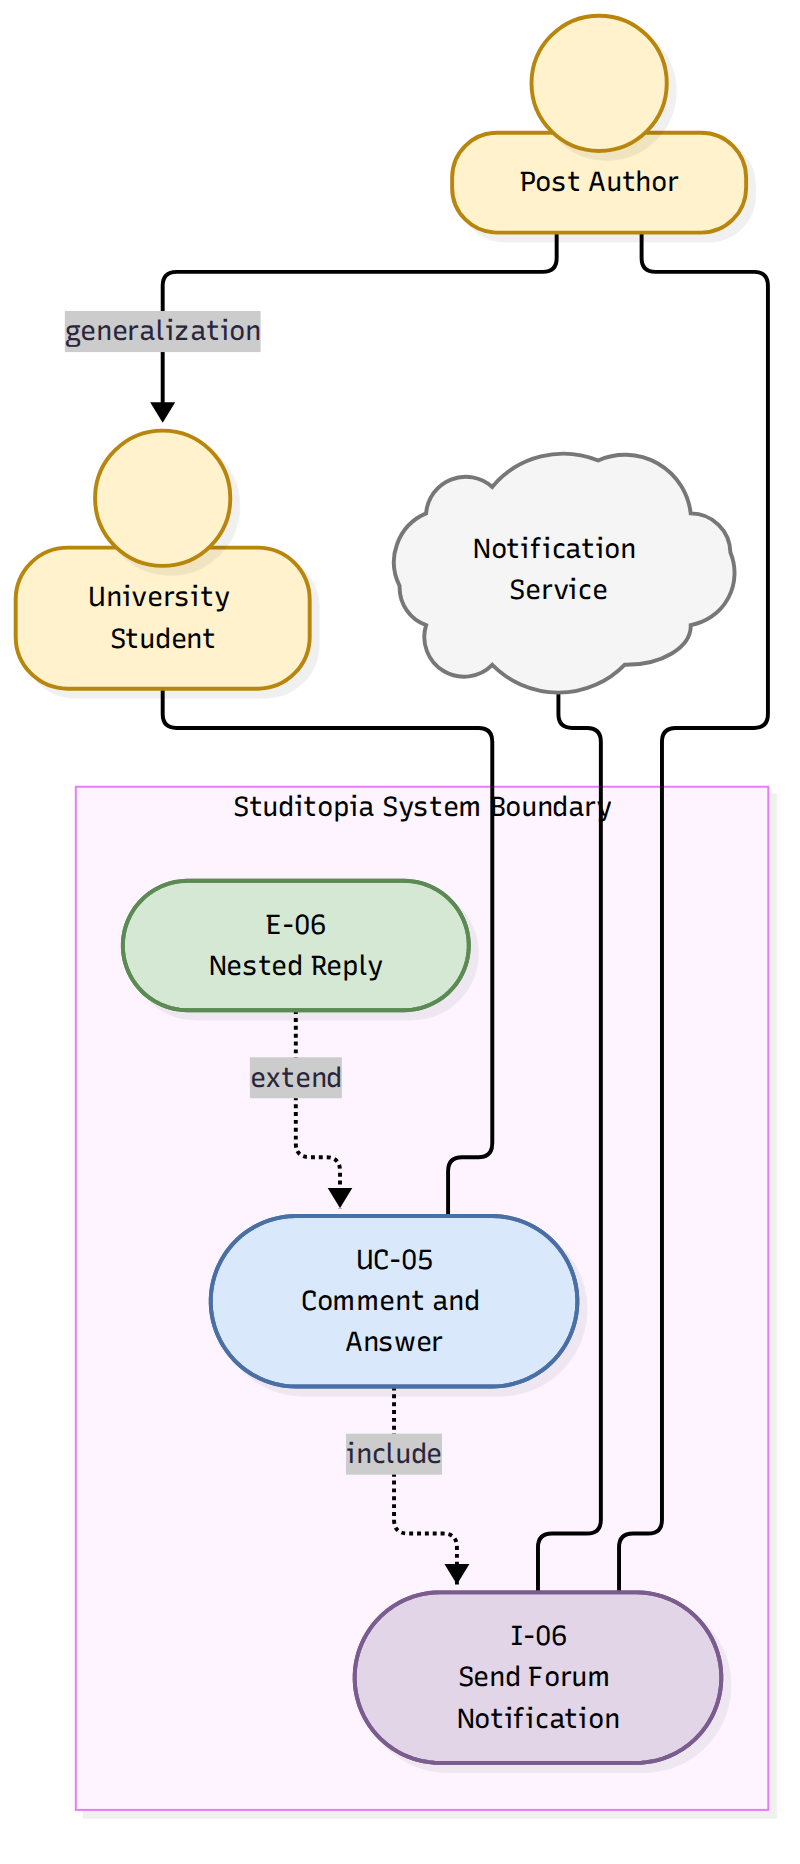
\includegraphics[width=0.85\textwidth,height=0.75\textheight,keepaspectratio]{figures/UC-05.png}
\end{center}
\par\medskip
\textbf{Diagram notation.} Person shape = human actor; cloud = supporting system; blue = selected base use case; purple = included; green = extending; solid line = association; dashed arrow = include or extend; labelled solid arrow = generalization.
\par\medskip
\hypertarget{sec:5-4-flow-of-events}{}
\addcontentsline{toc}{subsection}{5.4 Flow of Events}
\subsection*{5.4 Flow of Events}
\par\medskip
\hypertarget{sec:5-4-1-basic-flow}{}
\addcontentsline{toc}{subsubsection}{5.4.1 Basic Flow}
\subsubsection*{5.4.1 Basic Flow}
\par\medskip
\begin{enumerate}
\item The student opens a post detail page.
\item The system displays the post's existing comments and answers, including the marked true response when present.
\item The student selects the comment or answer composer.
\item The student enters the response content.
\item The system identifies whether the response is a comment on a discussion post or an answer to a question post.
\item The student submits the response.
\item The frontend validates that the response is not empty and submits it to the backend.
\item The backend verifies authentication, post visibility, posting permission, content validity, and rate limits.
\item The backend stores the comment or answer, associates it with the post and the student, and updates the discussion structure.
\item The system updates the displayed thread and comment or answer count.
\item The notification service notifies the post author that a new comment or answer was added.
\item The student sees the published response in the thread.
\end{enumerate}
\par\medskip
\hypertarget{sec:5-4-2-alternative-flows}{}
\addcontentsline{toc}{subsubsection}{5.4.2 Alternative Flows}
\subsubsection*{5.4.2 Alternative Flows}
\par\medskip
Unless otherwise stated, an alternative flow resumes at the next step of the basic flow.
\par\medskip
\hypertarget{sec:a1-nested-reply}{}
\paragraph*{A1. Nested reply}
\par\medskip
At basic flow step 4, the student replies to an existing comment or answer. The system stores the response with its parent and displays it in the threaded structure where applicable.
\par\medskip
\hypertarget{sec:a2-edit-own-response}{}
\paragraph*{A2. Edit own response}
\par\medskip
The student selects \textbf{Edit} on their own comment or answer, changes the content, and submits. The system validates and updates the existing response.
\par\medskip
\hypertarget{sec:a3-delete-own-response}{}
\paragraph*{A3. Delete own response}
\par\medskip
The student selects \textbf{Delete} on their own comment or answer and confirms. The system removes or hides the response according to the platform's deletion policy and updates the thread.
\par\medskip
\hypertarget{sec:a4-answer-a-question}{}
\paragraph*{A4. Answer a question}
\par\medskip
At basic flow step 5, the system classifies the response as an answer to the question post, making it eligible for true-response marking by the post author.
\par\medskip
\hypertarget{sec:a5-no-existing-discussion}{}
\paragraph*{A5. No existing discussion}
\par\medskip
At basic flow step 2, the system shows an empty discussion state and still presents the composer.
\par\medskip
\hypertarget{sec:e1-empty-or-invalid-response}{}
\paragraph*{E1. Empty or invalid response}
\par\medskip
The system keeps the composer open, shows validation feedback, and does not submit.
\par\medskip
\hypertarget{sec:e2-post-removed-locked-or-inaccessible}{}
\paragraph*{E2. Post removed, locked, or inaccessible}
\par\medskip
The system rejects the response and explains that the post is no longer available for discussion.
\par\medskip
\hypertarget{sec:e3-posting-restriction}{}
\paragraph*{E3. Posting restriction}
\par\medskip
A restricted or unauthorized student is denied commenting or answering.
\par\medskip
\hypertarget{sec:e4-rate-limit-reached}{}
\paragraph*{E4. Rate limit reached}
\par\medskip
The system rejects the response and asks the student to retry later.
\par\medskip
\hypertarget{sec:e5-notification-delivery-failure}{}
\paragraph*{E5. Notification delivery failure}
\par\medskip
The comment or answer remains published; the system records or retries the notification according to the notification policy.
\par\medskip
\hypertarget{sec:e6-server-or-database-failure}{}
\paragraph*{E6. Server or database failure}
\par\medskip
No response is stored, and the student receives a retry option with the entered content preserved where supported.
\par\medskip
\hypertarget{sec:5-4-3-business-rules}{}
\addcontentsline{toc}{subsubsection}{5.4.3 Business Rules}
\subsubsection*{5.4.3 Business Rules}
\par\medskip
\begin{enumerate}
\item Comments are allowed on discussion posts; answers are allowed on question posts.
\item Nested replies are supported where applicable.
\item Students may edit or delete only their own comments and answers.
\item Comments and answers are displayed in chronological or threaded order.
\item The post author is notified when a new comment or answer is added.
\item Commenting and answering are subject to authentication, permission, and rate-limit checks.
\item Only one true response may be marked for a question post; that action is performed by the post author under US-20.
\end{enumerate}
\par\medskip
\hypertarget{sec:5-5-special-requirements}{}
\addcontentsline{toc}{subsection}{5.5 Special Requirements}
\subsection*{5.5 Special Requirements}
\par\medskip
\begingroup
\small
\renewcommand{\baselinestretch}{1.0}\selectfont
\renewcommand{\arraystretch}{1.15}
\setlength{\tabcolsep}{6pt}
\begin{longtable}{|>{\raggedright\arraybackslash}p{0.22\textwidth}|>{\raggedright\arraybackslash}p{0.73\textwidth}|}
\hline
\textbf{ID} & \textbf{Requirement} \\ \hline
\endhead
NFR-PERF-4 & A new comment or answer must be reflected in the relevant forum view within 2 seconds. \\ \hline
NFR-PERF-6 & Forum notifications must be delivered with a latency of 2 seconds or less under normal operating conditions. \\ \hline
NFR-SEC-9 & Commenting and answering must be rate-limited to reduce spam and abuse. \\ \hline
Design constraint & A notification delivery failure must not roll back an already published comment or answer; the notification may be recorded or retried. \\ \hline
\end{longtable}
\endgroup
\par\medskip
\hypertarget{sec:5-6-preconditions}{}
\addcontentsline{toc}{subsection}{5.6 Preconditions}
\subsection*{5.6 Preconditions}
\par\medskip
\begin{enumerate}
\item The student is authenticated with an active session.
\item The student can view the selected post.
\item The post accepts comments or answers and has not been removed or locked.
\item The student is not restricted from commenting or answering.
\end{enumerate}
\par\medskip
\hypertarget{sec:5-7-postconditions}{}
\addcontentsline{toc}{subsection}{5.7 Postconditions}
\subsection*{5.7 Postconditions}
\par\medskip
\begin{enumerate}
\item \textbf{Success:} The comment or answer is stored and associated with the post, its author, and its parent comment when applicable.
\item \textbf{Success:} The comment or answer is displayed in the post's discussion in chronological or threaded order.
\item \textbf{Success:} The post author receives a notification about the new comment or answer.
\item \textbf{Failure:} No comment or answer is stored, and the student receives a clear error message.
\end{enumerate}
\par\medskip
\hypertarget{sec:5-8-extension-points}{}
\addcontentsline{toc}{subsection}{5.8 Extension Points}
\subsection*{5.8 Extension Points}
\par\medskip
\begingroup
\small
\renewcommand{\baselinestretch}{1.0}\selectfont
\renewcommand{\arraystretch}{1.15}
\setlength{\tabcolsep}{6pt}
\begin{longtable}{|>{\raggedright\arraybackslash}p{0.35\textwidth}|>{\raggedright\arraybackslash}p{0.6\textwidth}|}
\hline
\textbf{Extension Point} & \textbf{Location in Flow of Events} \\ \hline
\endhead
Nested reply & Basic flow step 4; alternative A1 \\ \hline
Edit or delete own response & After the response is displayed; alternatives A2-A3 \\ \hline
Answer classification & Basic flow step 5; alternative A4 \\ \hline
Empty discussion & Basic flow step 2; alternative A5 \\ \hline
Notification delivery & Basic flow step 11; exception E5 \\ \hline
Rate-limit recovery & Basic flow step 8; exception E4 \\ \hline
\end{longtable}
\endgroup
\par\medskip
\par\noindent\rule{\linewidth}{0.4pt}\par\medskip
\hypertarget{sec:6-uc-06-share-learning-resource}{}
\hypertarget{6-uc-06-share-learning-resource}{}
\addcontentsline{toc}{section}{6. UC-06 Share Learning Resource}
\section*{6. UC-06 Share Learning Resource}
\par\medskip
\hypertarget{sec:6-1-use-case-name}{}
\addcontentsline{toc}{subsection}{6.1 Use-Case Name}
\subsection*{6.1 Use-Case Name}
\par\medskip
\texttt{UC-06 Share Learning Resource}
\par\medskip
\hypertarget{sec:6-2-brief-description}{}
\addcontentsline{toc}{subsection}{6.2 Brief Description}
\subsection*{6.2 Brief Description}
\par\medskip
A student publishes a learning resource so that other students can discover and access useful academic material. The resource includes metadata, optional tags, and an uploaded file, and becomes searchable after publication.
\par\medskip
\begingroup
\small
\renewcommand{\baselinestretch}{1.0}\selectfont
\renewcommand{\arraystretch}{1.15}
\setlength{\tabcolsep}{6pt}
\begin{longtable}{|>{\raggedright\arraybackslash}p{0.28\textwidth}|>{\raggedright\arraybackslash}p{0.67\textwidth}|}
\hline
\textbf{Field} & \textbf{Value} \\ \hline
\endhead
Use Case ID & UC-06 \\ \hline
Primary Actor & University Student \\ \hline
Supporting Actors & None \\ \hline
Feature Group & Learning Resource Library \\ \hline
Priority & High \\ \hline
Related User Stories & US-27 \\ \hline
Related Requirements & FR-27.1 to FR-27.5; FR-25.1 to FR-25.5; FR-28.1 to FR-28.3; FR-29.1 to FR-29.4; NFR-SEC-5, NFR-PRIV-5, NFR-SCAL-4 \\ \hline
\end{longtable}
\endgroup
\par\medskip
\hypertarget{sec:6-3-use-case-diagram}{}
\addcontentsline{toc}{subsection}{6.3 Use Case Diagram}
\subsection*{6.3 Use Case Diagram}
\par\medskip
\begin{center}
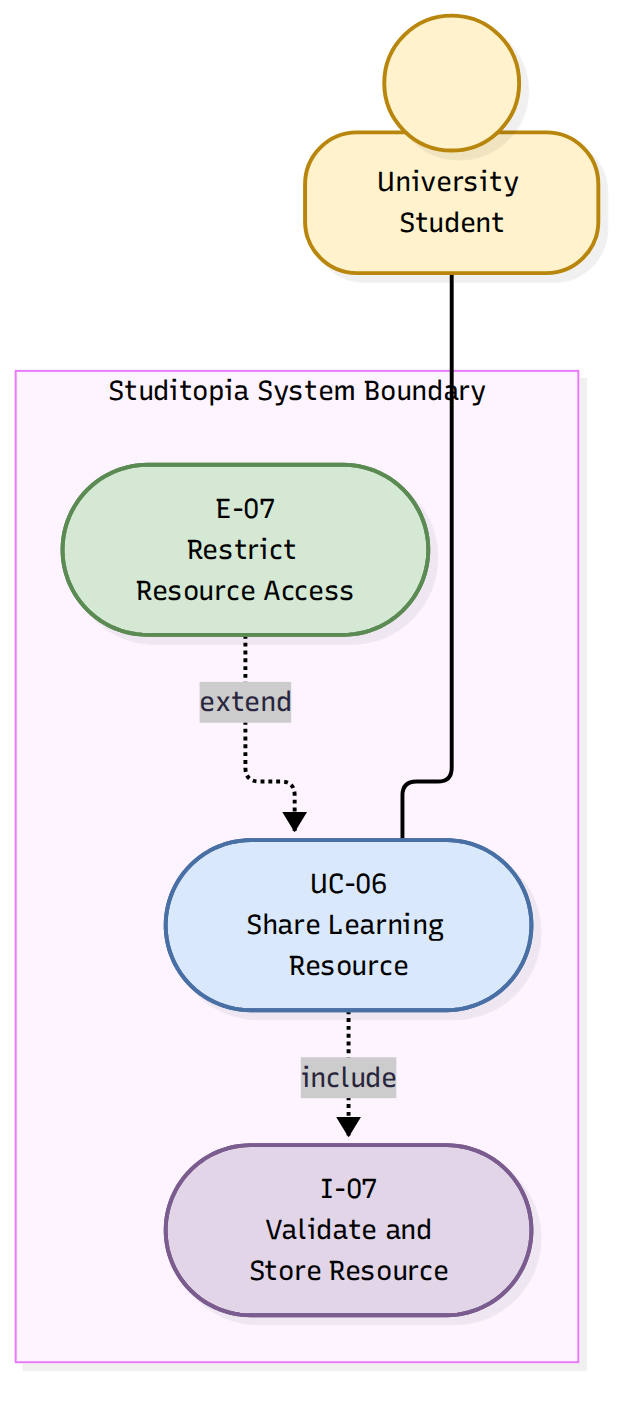
\includegraphics[width=0.85\textwidth,height=0.75\textheight,keepaspectratio]{figures/UC-06.png}
\end{center}
\par\medskip
\textbf{Diagram notation.} Person shape = human actor; blue = selected base use case; purple = included; green = extending; solid line = association; dashed arrow = include or extend.
\par\medskip
\hypertarget{sec:6-4-flow-of-events}{}
\addcontentsline{toc}{subsection}{6.4 Flow of Events}
\subsection*{6.4 Flow of Events}
\par\medskip
\hypertarget{sec:6-4-1-basic-flow}{}
\addcontentsline{toc}{subsubsection}{6.4.1 Basic Flow}
\subsubsection*{6.4.1 Basic Flow}
\par\medskip
\begin{enumerate}
\item The student opens the Learning Resource Library and selects \textbf{Share Resource}.
\item The system displays the resource form for title, description, subject tags, course tags, and file upload.
\item The student enters the resource details and selects a file.
\item The frontend validates the required fields and checks the file type and size against the configured limits.
\item The student submits the resource.
\item The backend verifies authentication and publication permission, validates the metadata and file, and performs the configured file-safety checks.
\item The backend stores the file and creates the resource record associated with the student, tags, and academic context.
\item The system publishes the resource and makes it searchable in the library.
\item The system displays a success confirmation and the resource in the student's storage view.
\item The resource becomes available to other users according to its privacy settings.
\end{enumerate}
\par\medskip
\hypertarget{sec:6-4-2-alternative-flows}{}
\addcontentsline{toc}{subsubsection}{6.4.2 Alternative Flows}
\subsubsection*{6.4.2 Alternative Flows}
\par\medskip
Unless otherwise stated, an alternative flow resumes at the next step of the basic flow.
\par\medskip
\hypertarget{sec:a1-add-or-change-tags}{}
\paragraph*{A1. Add or change tags}
\par\medskip
At basic flow step 3, the student adds or removes subject or course tags. The system updates the searchable metadata before publication.
\par\medskip
\hypertarget{sec:a2-replace-the-file-before-submission}{}
\paragraph*{A2. Replace the file before submission}
\par\medskip
The student selects a different file. The system revalidates file type and size and replaces the pending upload.
\par\medskip
\hypertarget{sec:a3-privacy-restricted-resource}{}
\paragraph*{A3. Privacy-restricted resource}
\par\medskip
At basic flow step 8, the resource is published with restricted access. It becomes searchable according to the privacy rule, but only authorized users can access the file.
\par\medskip
\hypertarget{sec:a4-cancel-publication}{}
\paragraph*{A4. Cancel publication}
\par\medskip
The student leaves the form before submitting. No published resource is created.
\par\medskip
\hypertarget{sec:a5-view-own-published-resources}{}
\paragraph*{A5. View own published resources}
\par\medskip
After publication, the student opens the storage view to see the resource status, publication date, and access statistics.
\par\medskip
\hypertarget{sec:e1-missing-or-invalid-metadata}{}
\paragraph*{E1. Missing or invalid metadata}
\par\medskip
The system highlights the invalid fields, keeps the form open, and does not publish.
\par\medskip
\hypertarget{sec:e2-unsupported-file-type-or-oversized-file}{}
\paragraph*{E2. Unsupported file type or oversized file}
\par\medskip
The system rejects the file, identifies the violated constraint, and allows the student to choose another file.
\par\medskip
\hypertarget{sec:e3-file-safety-check-fails}{}
\paragraph*{E3. File-safety check fails}
\par\medskip
The system blocks publication and informs the student that the file cannot be accepted.
\par\medskip
\hypertarget{sec:e4-storage-or-database-failure}{}
\paragraph*{E4. Storage or database failure}
\par\medskip
No published resource is created. The system displays a retry option and avoids leaving an orphaned or partially published resource.
\par\medskip
\hypertarget{sec:e5-publication-permission-lost}{}
\paragraph*{E5. Publication permission lost}
\par\medskip
The system rejects the publication and explains that the student is no longer authorized.
\par\medskip
\hypertarget{sec:e6-resource-becomes-unavailable-after-publication}{}
\paragraph*{E6. Resource becomes unavailable after publication}
\par\medskip
The system prevents further access and removes the resource from search and library listings when required.
\par\medskip
\hypertarget{sec:6-4-3-business-rules}{}
\addcontentsline{toc}{subsubsection}{6.4.3 Business Rules}
\subsubsection*{6.4.3 Business Rules}
\par\medskip
\begin{enumerate}
\item A resource must include a title and the metadata required for publication.
\item A resource can include a description, subject tags, and course tags.
\item Uploaded files must pass file type and size validation before acceptance.
\item A published resource must be searchable in the library.
\item Access to a published resource must follow the owner's privacy settings.
\item A deleted resource must be removed from search and library listings and must no longer be accessible to other users.
\item Publication is restricted to authenticated and authorized students.
\end{enumerate}
\par\medskip
\hypertarget{sec:6-5-special-requirements}{}
\addcontentsline{toc}{subsection}{6.5 Special Requirements}
\subsection*{6.5 Special Requirements}
\par\medskip
\begingroup
\small
\renewcommand{\baselinestretch}{1.0}\selectfont
\renewcommand{\arraystretch}{1.15}
\setlength{\tabcolsep}{6pt}
\begin{longtable}{|>{\raggedright\arraybackslash}p{0.22\textwidth}|>{\raggedright\arraybackslash}p{0.73\textwidth}|}
\hline
\textbf{ID} & \textbf{Requirement} \\ \hline
\endhead
NFR-SEC-5 & Uploaded files must be validated for file type and file size before acceptance. \\ \hline
NFR-PRIV-5 & Users must be able to control access to documents and learning resources they share. \\ \hline
NFR-SCAL-4 & The architecture must support at least 100,000 uploaded documents and learning resources. \\ \hline
Design constraint & Configured file-safety checks must complete before publication, and failed storage or database operations must not leave orphaned or partially published resources. \\ \hline
\end{longtable}
\endgroup
\par\medskip
\hypertarget{sec:6-6-preconditions}{}
\addcontentsline{toc}{subsection}{6.6 Preconditions}
\subsection*{6.6 Preconditions}
\par\medskip
\begin{enumerate}
\item The student is authenticated with an active session.
\item The student is permitted to publish resources to the library.
\item The file storage service and configured file-validation checks are available.
\end{enumerate}
\par\medskip
\hypertarget{sec:6-7-postconditions}{}
\addcontentsline{toc}{subsection}{6.7 Postconditions}
\subsection*{6.7 Postconditions}
\par\medskip
\begin{enumerate}
\item \textbf{Success:} A validated resource is stored with its owner, metadata, file, subject tags, and course tags.
\item \textbf{Success:} The resource is searchable in the library after publication.
\item \textbf{Success:} Other users can view and access the resource according to its privacy settings.
\item \textbf{Failure:} No resource is published, and the student receives a clear validation or system error.
\end{enumerate}
\par\medskip
\hypertarget{sec:6-8-extension-points}{}
\addcontentsline{toc}{subsection}{6.8 Extension Points}
\subsection*{6.8 Extension Points}
\par\medskip
\begingroup
\small
\renewcommand{\baselinestretch}{1.0}\selectfont
\renewcommand{\arraystretch}{1.15}
\setlength{\tabcolsep}{6pt}
\begin{longtable}{|>{\raggedright\arraybackslash}p{0.35\textwidth}|>{\raggedright\arraybackslash}p{0.6\textwidth}|}
\hline
\textbf{Extension Point} & \textbf{Location in Flow of Events} \\ \hline
\endhead
Tag changes & Basic flow step 3; alternative A1 \\ \hline
File replacement & Basic flow step 3; alternative A2 \\ \hline
Privacy restriction & Basic flow step 8; alternative A3 \\ \hline
Metadata validation failure & Basic flow step 4; exception E1 \\ \hline
File validation failure & Basic flow steps 4 and 6; exceptions E2-E3 \\ \hline
Cancel publication & Before basic flow step 5; alternative A4 \\ \hline
Storage-view review & Basic flow step 9; alternative A5 \\ \hline
\end{longtable}
\endgroup
\par\medskip
\par\noindent\rule{\linewidth}{0.4pt}\par\medskip
\hypertarget{sec:7-uc-07-join-or-create-a-study-room}{}
\hypertarget{7-uc-07-join-or-create-a-study-room}{}
\addcontentsline{toc}{section}{7. UC-07 Join or Create a Study Room}
\section*{7. UC-07 Join or Create a Study Room}
\par\medskip
\hypertarget{sec:7-1-use-case-name}{}
\addcontentsline{toc}{subsection}{7.1 Use-Case Name}
\subsection*{7.1 Use-Case Name}
\par\medskip
\texttt{UC-07 Join or Create a Study Room}
\par\medskip
\hypertarget{sec:7-2-brief-description}{}
\addcontentsline{toc}{subsection}{7.2 Brief Description}
\subsection*{7.2 Brief Description}
\par\medskip
A student enters an optional live study space by joining a public room, requesting access to a private room, or creating a new room for a study group. Meeting rooms are secondary supporting features and do not replace the forum as the primary collaboration space.
\par\medskip
\begingroup
\small
\renewcommand{\baselinestretch}{1.0}\selectfont
\renewcommand{\arraystretch}{1.15}
\setlength{\tabcolsep}{6pt}
\begin{longtable}{|>{\raggedright\arraybackslash}p{0.28\textwidth}|>{\raggedright\arraybackslash}p{0.67\textwidth}|}
\hline
\textbf{Field} & \textbf{Value} \\ \hline
\endhead
Use Case ID & UC-07 \\ \hline
Primary Actor & University Student \\ \hline
Supporting Actors & Room Owner or Manager; Notification Service \\ \hline
Feature Group & Meeting Rooms (Secondary) \\ \hline
Priority & Medium (Supporting) \\ \hline
Related User Stories & US-34, US-35 \\ \hline
Related Requirements & FR-34.1 to FR-34.4; FR-35.1 to FR-35.6; FR-36.1 to FR-36.6; FR-38.3; FR-39.3; NFR-PERF-7, NFR-SCAL-6, NFR-PRIV-6 \\ \hline
\end{longtable}
\endgroup
\par\medskip
\hypertarget{sec:7-3-use-case-diagram}{}
\addcontentsline{toc}{subsection}{7.3 Use Case Diagram}
\subsection*{7.3 Use Case Diagram}
\par\medskip
\begin{center}
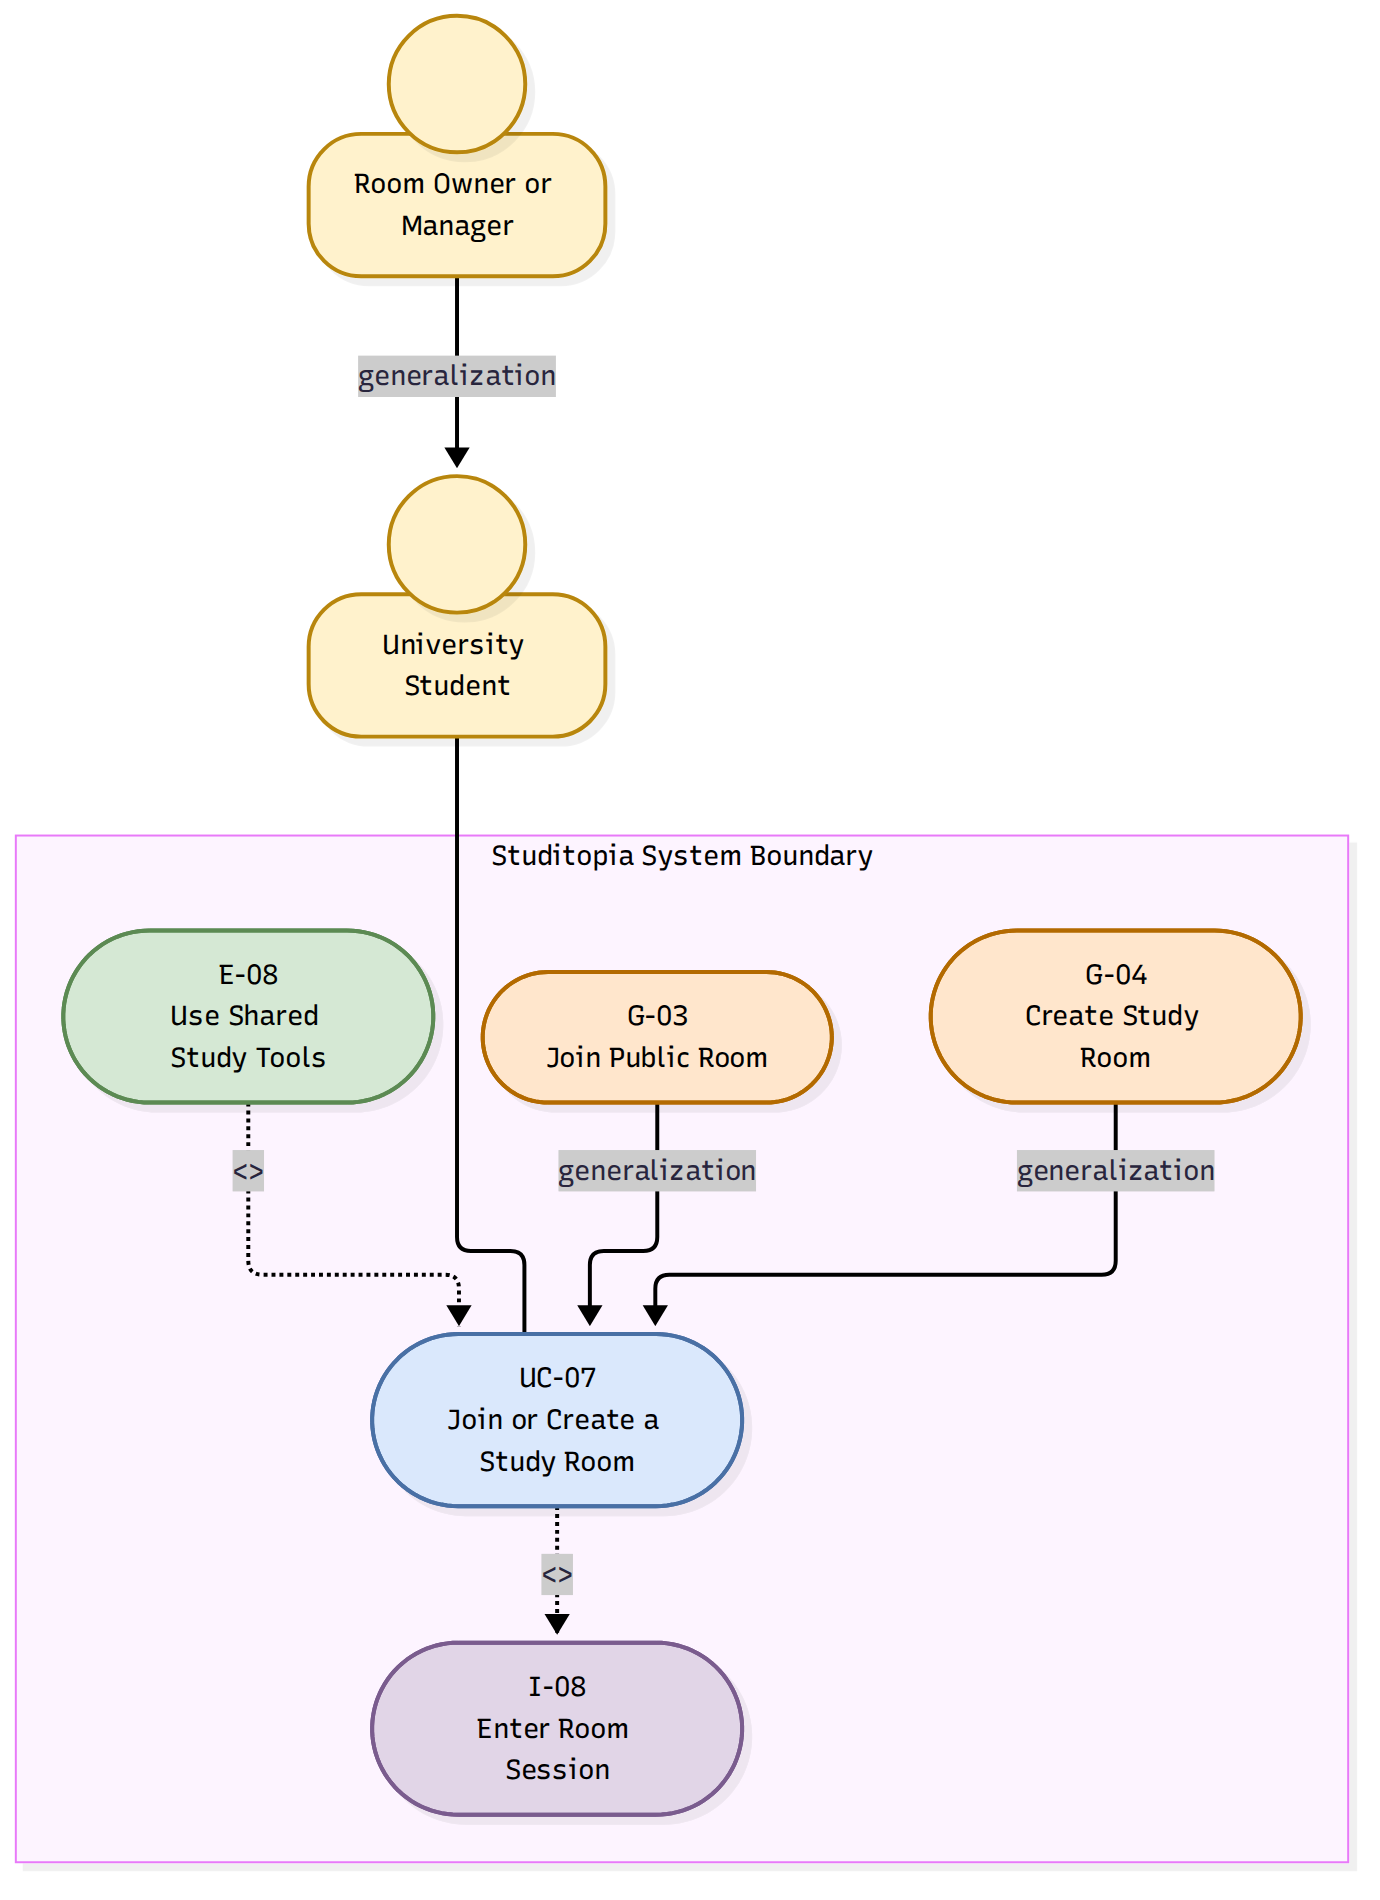
\includegraphics[width=0.85\textwidth,height=0.75\textheight,keepaspectratio]{figures/UC-07.png}
\end{center}
\par\medskip
\textbf{Diagram notation.} Person shape = human actor; cloud = supporting system; blue = selected base use case; purple = included; green = extending; orange = specialized; solid line = association; dashed arrow = include or extend; labelled solid arrow = generalization.
\par\medskip
\hypertarget{sec:7-4-flow-of-events}{}
\addcontentsline{toc}{subsection}{7.4 Flow of Events}
\subsection*{7.4 Flow of Events}
\par\medskip
\hypertarget{sec:7-4-1-basic-flow}{}
\addcontentsline{toc}{subsubsection}{7.4.1 Basic Flow}
\subsubsection*{7.4.1 Basic Flow}
\par\medskip
\begin{enumerate}
\item The student opens the Meeting Lobby.
\item The system displays available public study rooms with availability and capacity information.
\item The student selects a public room.
\item The backend verifies that the room still exists, is public, and has an available seat.
\item The backend adds the student to the room's participant list and establishes the room session.
\item The system opens the room and displays the supported shared study tools.
\item The student collaborates in the room using the available tools.
\end{enumerate}
\par\medskip
\hypertarget{sec:7-4-2-alternative-flows}{}
\addcontentsline{toc}{subsubsection}{7.4.2 Alternative Flows}
\subsubsection*{7.4.2 Alternative Flows}
\par\medskip
Unless otherwise stated, an alternative flow resumes at the next step of the basic flow.
\par\medskip
\hypertarget{sec:a1-request-a-private-room}{}
\paragraph*{A1. Request a private room}
\par\medskip
At basic flow step 3, the student selects a private or custom room. The system creates a join request and notifies the room owner or manager. If accepted, the student joins the room; if rejected, the student is notified and remains in the lobby.
\par\medskip
\hypertarget{sec:a2-create-a-room}{}
\paragraph*{A2. Create a room}
\par\medskip
The student selects \textbf{Create Room}, enters a name, description, privacy level, supported tools, capacity, duration, and communication rules, and submits. The backend validates the configuration, creates the room, assigns the student as owner or manager, and opens the room.
\par\medskip
\hypertarget{sec:a3-view-room-details-before-joining}{}
\paragraph*{A3. View room details before joining}
\par\medskip
The student opens the room detail page to review capacity, description, and configuration before joining or requesting access.
\par\medskip
\hypertarget{sec:a4-room-becomes-full}{}
\paragraph*{A4. Room becomes full}
\par\medskip
At basic flow step 4, the room has no available seat. The system prevents the join, explains that the room is full, and returns the student to the lobby.
\par\medskip
\hypertarget{sec:a5-use-shared-tools}{}
\paragraph*{A5. Use shared tools}
\par\medskip
After entering the room, the student uses the shared whiteboard, shared notes, or shared timer. Updates are synchronized for all participants.
\par\medskip
\hypertarget{sec:a6-reconnect-after-interruption}{}
\paragraph*{A6. Reconnect after interruption}
\par\medskip
If the room connection is interrupted, the system attempts to restore the session and preserve shared notes without data loss.
\par\medskip
\hypertarget{sec:e1-private-request-rejected}{}
\paragraph*{E1. Private request rejected}
\par\medskip
The owner or manager rejects the request. The student receives a notification and cannot enter the room.
\par\medskip
\hypertarget{sec:e2-room-no-longer-exists-or-is-closed}{}
\paragraph*{E2. Room no longer exists or is closed}
\par\medskip
The system informs the student and refreshes the lobby.
\par\medskip
\hypertarget{sec:e3-capacity-race-condition}{}
\paragraph*{E3. Capacity race condition}
\par\medskip
Another student takes the last seat before the join completes. The system rejects the join and shows that the room is full.
\par\medskip
\hypertarget{sec:e4-invalid-room-configuration}{}
\paragraph*{E4. Invalid room configuration}
\par\medskip
When creating or configuring a room, the system highlights invalid values such as unsupported capacity or duration and does not create the room.
\par\medskip
\hypertarget{sec:e5-real-time-service-failure}{}
\paragraph*{E5. Real-time service failure}
\par\medskip
The student cannot enter or remain in the live room. The system reports the failure and preserves shared notes where possible.
\par\medskip
\hypertarget{sec:e6-unauthorized-or-blocked-participant}{}
\paragraph*{E6. Unauthorized or blocked participant}
\par\medskip
The backend denies room entry and explains the access restriction.
\par\medskip
\hypertarget{sec:7-4-3-business-rules}{}
\addcontentsline{toc}{subsubsection}{7.4.3 Business Rules}
\subsubsection*{7.4.3 Business Rules}
\par\medskip
\begin{enumerate}
\item Meeting rooms are optional supporting features; they do not replace the forum as the primary collaboration space.
\item A public room can be joined when it has available capacity.
\item A private or custom room requires a join request that the owner or manager can accept or reject.
\item A room creator becomes the room owner or manager.
\item Room managers can configure capacity, duration, communication rules, privacy level, and supported tools.
\item Shared tool updates must be synchronized for all room participants.
\item Shared notes must be preserved during the room session and handle reconnection without data loss.
\item Room participation and invitations must respect the user's communication and privacy settings.
\end{enumerate}
\par\medskip
\hypertarget{sec:7-5-special-requirements}{}
\addcontentsline{toc}{subsection}{7.5 Special Requirements}
\subsection*{7.5 Special Requirements}
\par\medskip
\begingroup
\small
\renewcommand{\baselinestretch}{1.0}\selectfont
\renewcommand{\arraystretch}{1.15}
\setlength{\tabcolsep}{6pt}
\begin{longtable}{|>{\raggedright\arraybackslash}p{0.22\textwidth}|>{\raggedright\arraybackslash}p{0.73\textwidth}|}
\hline
\textbf{ID} & \textbf{Requirement} \\ \hline
\endhead
NFR-PERF-7 & Optional supporting meeting-room tools must maintain an update latency of 1 second or less when a room is in use. \\ \hline
NFR-SCAL-6 & The architecture must support at least 100 concurrent optional meeting rooms. \\ \hline
NFR-PRIV-6 & Users must be able to control whether other users can send them messages or room invitations. \\ \hline
Design constraint & Shared tool updates must be synchronized for all participants, and shared notes must be preserved during reconnection without data loss. Meeting rooms remain secondary to the forum. \\ \hline
\end{longtable}
\endgroup
\par\medskip
\hypertarget{sec:7-6-preconditions}{}
\addcontentsline{toc}{subsection}{7.6 Preconditions}
\subsection*{7.6 Preconditions}
\par\medskip
\begin{enumerate}
\item The student is authenticated with an active session.
\item The meeting-room service and real-time collaboration service are available.
\item The student is permitted to access the study-room lobby and is not blocked from room participation.
\item A room is available, or the student is permitted to create one.
\end{enumerate}
\par\medskip
\hypertarget{sec:7-7-postconditions}{}
\addcontentsline{toc}{subsection}{7.7 Postconditions}
\subsection*{7.7 Postconditions}
\par\medskip
\begin{enumerate}
\item \textbf{Success:} The student joins a room with an available seat, or creates a room and becomes its owner or manager.
\item \textbf{Success:} The student can enter the room and use supported shared study tools according to the room configuration.
\item \textbf{Success:} Room join requests are routed to an owner or manager for a private or custom room.
\item \textbf{Failure:} The student remains outside the room and receives a clear reason, such as full capacity, rejected request, or unavailable room.
\end{enumerate}
\par\medskip
\hypertarget{sec:7-8-extension-points}{}
\addcontentsline{toc}{subsection}{7.8 Extension Points}
\subsection*{7.8 Extension Points}
\par\medskip
\begingroup
\small
\renewcommand{\baselinestretch}{1.0}\selectfont
\renewcommand{\arraystretch}{1.15}
\setlength{\tabcolsep}{6pt}
\begin{longtable}{|>{\raggedright\arraybackslash}p{0.35\textwidth}|>{\raggedright\arraybackslash}p{0.6\textwidth}|}
\hline
\textbf{Extension Point} & \textbf{Location in Flow of Events} \\ \hline
\endhead
Private-room request & Basic flow step 3; alternative A1 \\ \hline
Create room & Meeting Lobby; alternative A2 \\ \hline
View room details & Before joining or requesting access; alternative A3 \\ \hline
Room capacity check & Basic flow step 4; alternative A4 and exception E3 \\ \hline
Shared study tools & Basic flow steps 6-7; alternative A5 \\ \hline
Reconnect after interruption & During a room session; alternative A6 and exception E5 \\ \hline
Join-request notification & Private-room request and decision; alternative A1 and exception E1 \\ \hline
\end{longtable}
\endgroup
\par\medskip

\end{document}
